\documentclass[11pt]{article}

\usepackage[margin=1in]{geometry}
\usepackage{amsmath,amssymb,amsthm}
\usepackage{booktabs}
\usepackage{enumitem}
\usepackage{microtype}
\usepackage{needspace}
\usepackage{xcolor}
\usepackage{tikz}
\usepackage{hyperref}
\usepackage[nameinlink,noabbrev]{cleveref}

\hypersetup{
  colorlinks=true,
  linkcolor=blue!55!black,
  citecolor=green!45!black,
  urlcolor=blue!55!black
}

\newtheorem{theorem}{Theorem}[section]
\newtheorem{lemma}[theorem]{Lemma}
\newtheorem{proposition}[theorem]{Proposition}
\newtheorem{corollary}[theorem]{Corollary}
\theoremstyle{definition}
\newtheorem{definition}[theorem]{Definition}
\newtheorem{example}[theorem]{Example}
\newtheorem{question}[theorem]{Open Question}
\theoremstyle{remark}
\newtheorem{remark}[theorem]{Remark}

\crefname{question}{Open Question}{Open Questions}

\newcommand{\Rper}{\mathcal R_{\mathrm{per}}}
\newcommand{\Rbullet}{\mathcal R_{\mathrm{per}}^{\bullet}}
\newcommand{\Oper}{\mathcal O_{\mathrm{per}}}
\newcommand{\Obs}{\operatorname{Obs}_{\mathrm{pc}}}
\newcommand{\idim}{\operatorname{idim}}
\newcommand{\strc}{\operatorname{str}}
\newcommand{\sstrc}{\operatorname{sstr}}
\newcommand{\calF}{\mathcal F}
\newcommand{\eps}{\varepsilon}
\newcommand{\bits}{\{0,1\}}

\title{Convex-Treelike Partial Cubes:\\
Peripheral Recursion and Forbidden Minors}
\author{Olivier Bousquet}
\date{}

\begin{document}
\maketitle

\begin{abstract}
A tree-like partial cube is built from one vertex by peripheral expansions:
each step duplicates an isometric subgraph of the graph already constructed.
The duplicated subgraph need not itself be tree-like, so this class is not
closed under convex subgraphs. Polat's convex-treelike partial cubes require
every finite nontrivial convex subgraph to have a periphery. We characterize
the finite members by the stronger peripheral recursion in which both the
contraction base and the duplicated subgraph admit the same construction.

We prove that this class is closed under partial-cube minors and is the
largest such subclass of the tree-like partial cubes. Its description as
the largest convex-subgraph-closed subclass follows from Polat's
characterization. Here partial-cube minors use coordinate
projection and restriction to convex subgraphs. We then characterize
membership and minimal forbidden minors for one-vertex amalgams. The relevant
pointed factors are those whose peripheral decompositions can be chosen to
remove sides avoiding the identified vertex. Minimal failures of this
pointed property generate exactly the one-vertex-decomposable obstructions.

The forbidden minors with nonample vertex sets are precisely the cubes with
two antipodal vertices deleted. For the remaining, ample obstructions, we
give exact coordinate recognition criteria and express the effect of
projection through minimal sets of coordinates that repair a failed section
containment. We also give explicit obstructions and computer-assisted
small-order classifications. The recognition criteria may inspect all
coordinate states; a simpler intrinsic generator for the full forbidden
family remains open.
\end{abstract}

\section{Introduction}

Expansion is one of the fundamental ways to construct a partial cube.
Contracting a Djokovi\'c--Winkler class deletes one intrinsic hypercube
coordinate; reversing the contraction splits a graph along two isometric
covering subgraphs and adds a new matching.  Classical restrictions on the
overlap lead to median, almost-median, and semi-median graphs
\cite{ImrichKlavzar98,BresarImrichKlavzar03fast}.  A different restriction
is \emph{peripherality}: one member of the cover is the entire base graph.
Bre\v{s}ar, Imrich, and Klav\v{z}ar used sequences of such expansions to
define the tree-like partial cubes \cite{BresarImrichKlavzar03}.

There is a quantifier hidden in that definition.  A sequential construction
records only one chain of contraction bases.  The second member of a
peripheral cover---the site duplicated by the new coordinate---need not have
a compatible peripheral construction.  This distinction matters
structurally.  Tree-like partial cubes are closed under gated subgraphs, but
not under convex subgraphs \cite{Polat12treelike,Gologranc14treehamming}; in fact every
finite partial cube occurs as a convex semicube of some tree-like partial
cube.  Hence the standard tree-like class cannot be characterized by
forbidden partial-cube minors.

Polat introduced \emph{convex-treelike partial cubes}: every finite
nontrivial convex subgraph must have a periphery
\cite[Definition~5.5]{Polat12treelike}. He also proved that this is
equivalent to requiring every finite convex subgraph to be tree-like
\cite[Proposition~5.6]{Polat12treelike}. Throughout this paper our graphs
are finite.

We study this established class through a recursive construction and its
forbidden partial-cube minors. Starting with \(K_1\), allow a
peripheral expansion only when both its contraction base and its duplicated
site have already been constructed by the same rule.  We denote the resulting
class by \(\Rper\).
We use \emph{cover-recursive peripheral} to describe this construction;
\cref{thm:convex-characterization} identifies its members with the finite
convex-treelike partial cubes. The
requirement is motivated by the established distinction between sequential
and cover-recursive expansion classes: for example,
proper semi-median graphs require both cover members recursively, whereas
the isometric-expansion class uses only one expansion sequence
\cite{journals/jgt/BresarIKMS02}.

\paragraph{Main results.}
Our first theorem shows that the recursive condition supplies exactly the
heredity missing from the standard tree-like class.

\begin{theorem}[Hereditary characterization; informal form]
\label{thm:intro-characterization}
For a finite partial cube \(G\), the following are equivalent:
\begin{enumerate}[label=\textup{(\roman*)}]
  \item \(G\in\Rper\);
  \item every nontrivial partial-cube minor of \(G\) has a peripheral
        coordinate;
  \item every partial-cube minor of \(G\) is tree-like;
  \item every nontrivial convex subgraph of \(G\) has a peripheral
        coordinate; and
  \item every convex subgraph of \(G\) is tree-like.
\end{enumerate}
\end{theorem}

The equivalence of (iv) and (v) is Polat's characterization. We first identify
his class with the recursive construction: a convex subgraph that meets both
layers of a peripheral expansion inherits that expansion. We then commute
coordinate contraction past one peripheral step. These two arguments give
\cref{thm:convex-characterization,lem:pcminor-closure}; the pc-minor tests
are consequences. Expansion trees record the recursive construction.

Our second structural result concerns gluing at a vertex. A peripheral
decomposition of a pointed graph is \emph{root-avoiding} if each removed
peripheral side omits the root and this condition continues on the
contraction base. The duplicated site needs only an ordinary decomposition.
For two members of \(\Rper\), their one-vertex amalgam belongs to \(\Rper\)
if and only if at least one factor has a root-avoiding decomposition at the
identified vertex. Moreover, the amalgam is a minimal forbidden pc-minor
if and only if both factors are minimal failures of that pointed property
under root-preserving minors; see \cref{thm:rooted-wedge}. This gives a
construction of all one-vertex-decomposable obstructions. It also provides
an explicit failure of closure under gated amalgamation.

The class contains every median graph and every daisy cube, and all its
members are tree-like, ample, and corner-peelable. Here an ample class is a
vertex family whose shattered coordinate sets are exactly the coordinate
sets of its contained cubes. A corner peeling successively deletes vertices
lying in a unique maximal cube; the equivalent isometric-ordering convention
is fixed in \cref{sec:preliminaries}. The inclusions and separating examples
are collected in \cref{sec:position,sec:closure,sec:obstructions}.

The forbidden family has both a structural and an algorithmic description.
Its nonample members are exactly
\(Q_n^{--}=Q_n-\{x,\bar x\}\), \(n\ge3\). Every other forbidden minor is
ample. The sixteen-vertex pentagonal class \(\mathcal P_5\) is an explicit
example; its global vertex-minimality among these additional obstructions
is computer-assisted. The one-vertex construction gives a twenty-one-vertex
example from two eleven-vertex pointed factors.

For recognition, assign each coordinate one of four instructions: retain,
project, fix to zero, or fix to one. A nontrivial irredundant partial cube
is forbidden exactly when it has no peripheral coordinate and every proper
nontrivial resulting minor has one. This follows from the hereditary
characterization. The later two-layer formulation records witnesses to
failed section containments and the minimal coordinate sets whose
projection repairs them. These are exact tests, potentially over
exponentially many coordinate states. They do not yet give a succinct
intrinsic generator comparable to a decomposition into a few elementary
constructions.

\paragraph{Results at a glance.}
The paper separates equivalent characterizations from consequences and from
finite computations.  The following table records what each part contributes.
\begin{center}
\small
\begin{tabular}{@{}p{0.22\textwidth}p{0.53\textwidth}p{0.16\textwidth}@{}}
\toprule
Viewpoint & What it provides & Location \\
\midrule
Expansions
  & Binary peripheral expansion trees, and the precise distinction from a
    sequential tree-like construction
  & \Cref{sec:expansion-characterization} \\
Convex subgraphs
  & Identification with Polat's class and its convex-subgraph test
  & \Cref{sec:convex-characterization} \\
Pc-minors
  & Heredity and the test that every nontrivial pc-minor exposes a peripheral
    class
  & \Cref{sec:pcminor-characterization} \\
Forbidden basis
  & A coordinate recognition criterion and the nonample family; later,
    two-layer recognition and repair antichains
  & \Cref{sec:complete-basis,sec:repair-recognition} \\
Structure and examples
  & Class containments, closure properties, explicit obstructions, and the
    exact one-vertex-amalgam theorem
  & \Cref{sec:position,sec:closure,sec:obstructions,sec:wedges} \\
Finite verification
  & Finite classifications, enumeration domains, and verification methods
  & \Cref{sec:computation} \\
\bottomrule
\end{tabular}
\end{center}

\paragraph{Provenance and computation.}
The expansion, tree-like, pc-minor, ample, and corner-peeling results quoted
as background are explicitly attributed to their sources. The class
definition and the equivalence of the two convex-subgraph tests are due to
Polat; the largest convex-hereditary subclass statement is a consequence of
that equivalence. We give proofs of the recursive and pc-minor
characterizations, the rooted-wedge theorem, the obstruction minimality
arguments, and the small-order lemma. Polat's pointed example already
contains the factor used in our twenty-one-vertex obstruction; we explain
the relation and extend his construction in \cref{sec:polat-construction}.
Finite uniqueness and
small-order assertions are computer-assisted.  The enumeration is exhaustive
up to cube isomorphism and is documented in
\cref{sec:computation}.  Symbolic proofs do not rely on the enumeration unless
a statement is explicitly labelled computer-assisted.

\paragraph{Reading guide.}
\Cref{sec:preliminaries} fixes the partial-cube, minor, expansion, and
set-system language.  \Cref{sec:expansion-characterization} gives the
expansion-tree characterization and separates it from the usual sequential
tree-like construction.  \Cref{sec:convex-characterization} identifies the recursion with Polat's
class, and \cref{sec:pcminor-characterization} adds contraction closure
and the pc-minor characterization.
\Cref{sec:complete-basis} gives coordinate recognition and identifies the
nonample obstructions.  \Cref{sec:position} positions the
class among established classes, and \cref{sec:closure} collects its closure
and inherited properties.  \Cref{sec:obstructions} gives explicit ample
obstructions and the global small-order result.  \Cref{sec:wedges} treats
gated and one-vertex amalgams.
The main structural arguments can be read without the later repair
machinery: \cref{sec:repair-recognition} develops that coordinate test after
the examples and wedge theorem. \Cref{sec:computation} explains the finite
enumerations, and \cref{sec:conclusion} states the remaining generator
problem.

\section{Preliminaries}
\label{sec:preliminaries}

All graphs and coordinate sets are finite.  Graphs are simple and connected
unless stated otherwise.  For a graph \(G\), let \(d_G\) denote its shortest
path metric and
\[
 I_G(u,v)=\{w:d_G(u,w)+d_G(w,v)=d_G(u,v)\}
\]
its interval.  A vertex set \(S\) is \emph{convex} if
\(I_G(u,v)\subseteq S\) for all \(u,v\in S\); it is \emph{gated} if every
vertex \(x\) has a unique \(g\in S\) such that
\[
 d_G(x,s)=d_G(x,g)+d_G(g,s)\qquad(s\in S).
\]
Gated subgraphs are convex, and convex subgraphs are isometric.

\subsection{Coordinates, sections, and partial-cube minors}

The \(X\)-dimensional hypercube \(Q_X\) has vertex set \(\bits^X\) and
Hamming distance.  A \emph{partial cube} is a graph admitting an isometric
embedding into a hypercube.  We always suppress constant coordinates, so the
embedding is irredundant.

For edges \(xy\) and \(uv\), the Djokovi\'c--Winkler relation is
\[
 xy\mathrel\Theta uv
 \quad\Longleftrightarrow\quad
 d(x,u)+d(y,v)\ne d(x,v)+d(y,u).
\]
In a partial cube this is an equivalence relation.  Its classes are exactly
the edge sets that change one coordinate in an irredundant embedding; their
number is the \emph{isometric dimension} \(\idim(G)\).

Fix an embedding \(V(G)\subseteq\bits^X\).  For \(x\in X\) and
\(\eps\in\bits\), the two semicubes and their boundaries are
\[
 W_x^\eps=\{v:v_x=\eps\},\qquad
 U_x^\eps=\{v\in W_x^\eps:v\text{ has a neighbor in }W_x^{1-\eps}\}.
\]
The semicubes are complementary and convex.  Identifying a binary vector
with its support gives a family \(H\subseteq2^X\).  After deleting coordinate
\(x\), its two sections and its projection are
\[
 H_x^\eps=\{h\setminus\{x\}:h\in H,\ \mathbf1_{x\in h}=\eps\},
 \qquad
 \pi_xH=H_x^0\cup H_x^1.
\]
Restricting \(G\) to \(W_x^\eps\) gives the graph of \(H_x^\eps\), while
contracting the entire \(x\)-class gives the graph of \(\pi_xH\).

\begin{definition}[Peripheral coordinate]
\label{def:peripheral-coordinate}
A \(\Theta\)-class \(x\) is \emph{peripheral} if
\(U_x^\eps=W_x^\eps\) for at least one \(\eps\in\bits\).  Equivalently, its
projected sections are nested:
\[
 H_x^\eps\subseteq H_x^{1-\eps}
\]
for one orientation.  The smaller semicube is a \emph{periphery}.  A
nontrivial partial cube with no peripheral class is \emph{periphery-free}.
\end{definition}

\begin{definition}[Partial-cube minor]
\label{def:pcminor}
A \emph{restriction} of \(G\) is a nonempty convex subgraph.  The
\emph{contraction} \(G/E\) of a \(\Theta\)-class \(E\) simultaneously
identifies the endpoints of all edges of \(E\) and takes the simple quotient.
A \emph{partial-cube minor}, or \emph{pc-minor}, is obtained by a finite
sequence of restrictions and \(\Theta\)-class contractions.  It is
\emph{proper} if it is not isomorphic to \(G\).
\end{definition}

It suffices to use elementary restrictions to one semicube and contractions
of one class \cite[Section~2.1]{KnauerMarc20}.  Every convex subgraph of a
finite partial cube is an intersection of semicubes.  In set-family language,
the elementary operations are \(H_x^\eps\) and \(\pi_xH\), respectively.

\subsection{Shattering and neighboring graph classes}

For \(H\subseteq2^X\) and \(T\subseteq X\), the trace is
\(H|_T=\{h\cap T:h\in H\}\).  The family \(H\) \emph{shatters} \(T\) when
\(H|_T=2^T\), and \emph{strongly shatters} \(T\) when it contains a
\(T\)-dimensional cube with all other coordinates fixed.  Write
\[
 \strc(H)=\{T:H\text{ shatters }T\},\qquad
 \sstrc(H)=\{T:H\text{ strongly shatters }T\}.
\]
The VC dimension is the largest size of a shattered set.  The sandwich
inequalities are
\[
 |\sstrc(H)|\le |H|\le|\strc(H)|.
\]
A family is \emph{ample}, or \emph{lopsided}, when equality holds,
equivalently when \(\sstrc(H)=\strc(H)\)
\cite{BandeltCDK06}.  A VC-dimension-\(r\) family on \(n\) coordinates is
\emph{maximum} when it has \(\sum_{i=0}^r\binom ni\) members.  Every maximum
family is ample.

The \emph{crossing graph} \(G^\sharp\) has the \(\Theta\)-classes as vertices;
two are adjacent when all four intersections of their semicubes are
nonempty, equivalently when their coordinate pair is shattered.  For an
ample partial cube this agrees with the graph recording pairs realized by a
square.

We shall compare \(\Rper\) with the following established classes.
\begin{itemize}[leftmargin=2em]
  \item A partial cube is \emph{median} if, for every three vertices
        \(u,v,w\), the intersection
        \(I_G(u,v)\cap I_G(v,w)\cap I_G(w,u)\) has exactly one vertex.
  \item It is \emph{almost-median}, respectively \emph{semi-median}, if every
        boundary graph \(G[U_x^\eps]\) is isometric, respectively connected.
  \item It is \emph{proper semi-median} if it is semi-median and admits a
        connected expansion cover (one with connected overlap) whose two members recursively have the
        same property, beginning with \(K_1\)
        \cite[Section~3, class~(10)]{journals/jgt/BresarIKMS02}.
  \item It is a \emph{daisy cube} if, after choosing a root and orientations
        of the coordinates, its vertex family is a down-set in \(2^X\).
\end{itemize}

For an ample family, call an ordering \(v_1,\ldots,v_m\)
\emph{prefix-isometric} when every induced prefix
\(\{v_1,\ldots,v_i\}\) is isometric.  Chalopin, Chepoi, Moran, and Warmuth
prove that these are exactly the corner-peeling orderings of an ample family
\cite[Proposition~4.2]{ChalopiChepoiMoran22}.  We use this equivalence as the
definition-independent meaning of \emph{corner-peelable}.  Following that
source, an ample partial cube admitting such an ordering is also called
\emph{dismantlable ample}; this is unrelated to closed-neighborhood
dismantlability for general graphs.

Reversing a prefix-isometric ordering gives the order in which corners are
deleted. Statements about a corner peeling \emph{ending} at a specified
vertex use this deletion order; the corresponding prefix ordering begins
at that vertex.

\begin{example}[Three small coordinate models]
\label{ex:small-models}
The path \(P_4\), the cycle \(C_6\), and the cube \(Q_3\) have the
representations
\[
\begin{array}{c|c|c|c}
G&H&\idim(G)&G^\sharp\\ \hline
P_4&\{\varnothing,\{1\},\{1,2\},[3]\}&3&\overline K_3\\
C_6&2^{[3]}\setminus\{\varnothing,[3]\}&3&K_3\\
Q_3&2^{[3]}&3&K_3.
\end{array}
\]
The \(6\)-cycle shatters every coordinate pair but contains no square.  It
is the smallest antipodally punctured cube \(Q_3^{--}\) and is
periphery-free.  The cube is recursively peripheral, yet contains this
\(C_6\) as an induced isometric subgraph.
\end{example}

\subsection{Expansion and its quantifiers}

\begin{definition}[Expansion]
\label{def:expansion}
An \emph{expansion cover} of a connected graph \(B\) is a pair of isometric
induced subgraphs \(B_0,B_1\) such that
\[
 V(B)=V(B_0)\cup V(B_1),\qquad
 E(B)=E(B_0)\cup E(B_1),\qquad
 V(B_0)\cap V(B_1)\ne\varnothing.
\]
The corresponding \emph{expansion} takes disjoint copies of \(B_0,B_1\) and
joins the two copies of every vertex in \(B_0\cap B_1\).  It is
\emph{peripheral} when one cover member is the whole base \(B\).
\end{definition}

The expansion is \emph{connected} when its overlap \(B_0\cap B_1\) is
connected, and \emph{isometric} when that overlap is isometric in \(B\).
The latter condition is stronger than requiring the two cover members to
be isometric, which is part of every expansion cover here.

Every finite partial cube is obtained from \(K_1\) by expansions, reversing
a complete sequence of \(\Theta\)-class contractions
\cite[Theorem~3.1]{ImrichKlavzar98}.  In a peripheral expansion, orient the
new coordinate so that
\begin{equation}
 V(G)=(V(B)\times\{0\})\cup(V(S)\times\{1\}),
 \qquad S\subseteq B,
 \label{eq:peripheral-form}
\end{equation}
where the duplicated site \(S\) is isometric in \(B\).

There are two ways to generate a class from this operation.
\begin{definition}[Sequential and cover-recursive peripheral constructions]
\label{def:sequential-recursive}
A \emph{sequential peripheral construction} is a chain
\[
 K_1=G_0\longrightarrow G_1\longrightarrow\cdots\longrightarrow G_m=G
\]
of peripheral expansions.  The graphs admitting such a construction are the
standard \emph{tree-like partial cubes} \cite{BresarImrichKlavzar03}.

The \emph{cover-recursive peripheral class} \(\Rper\) is the least class
containing \(K_1\) such that a graph in the form
\eqref{eq:peripheral-form} belongs to \(\Rper\) whenever both \(B\) and \(S\)
belong to \(\Rper\).
\end{definition}

By \cref{thm:convex-characterization}, \(\Rper\) is precisely the finite
convex-treelike class of \cite[Definition~5.5]{Polat12treelike}. We retain
the recursive notation to make the two-child construction explicit.

Equivalently, a nontrivial partial cube \(G\) belongs to \(\Rper\) when
\emph{there exists} a peripheral coordinate \(e\) for which both the
contraction \(G/e\) and the duplicated site belong to \(\Rper\).  Only one
coordinate is required to witness a recursive step.  The requirement is not
universal over the peripheral coordinates, much less over all coordinates.
The recursion is instead universal over the two children of each chosen
step.  Thus its witness is a rooted binary tree, whereas a tree-like witness
is one distinguished path of contraction bases.

\begin{center}
\small
\begin{tabular}{@{}p{0.26\textwidth}p{0.28\textwidth}p{0.36\textwidth}@{}}
\toprule
Class & Witness & Requirement at one peripheral step\\
\midrule
tree-like partial cubes
  & one path of contraction bases
  & the contraction base continues the path; no recursive condition is
    imposed on the duplicated site\\
\(\Rper\)
  & a rooted binary tree
  & both the contraction base and the duplicated site recursively belong
    to \(\Rper\)\\
\bottomrule
\end{tabular}
\end{center}

\begin{example}[A square with an attached edge]
\label{ex:peripheral-step}
Take the path \(B=\{00,10,11\}\) and its edge \(S=\{00,10\}\). Duplicating
\(S\) gives
\[
 G=\{000,100,110,001,101\}.
\]
The last coordinate is peripheral: its one-section is \(S\), contained
in its zero-section \(B\). Projecting that coordinate recovers \(B\);
conditioning it to one recovers \(S\). Both are paths and admit recursive
peripheral decompositions, so \(G\in\Rper\).
\begin{center}
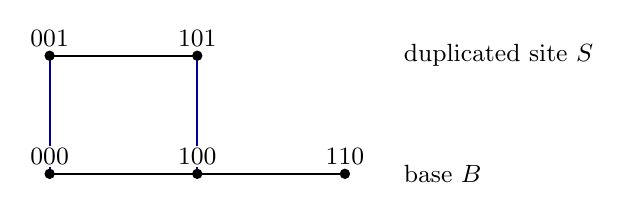
\begin{tikzpicture}[scale=1.25,every node/.style={font=\small}]
 \draw[thick] (0,0)--(1.5,0)--(3,0);
 \draw[thick] (0,1.2)--(1.5,1.2);
 \draw[thick,blue!60!black] (0,0)--(0,1.2) (1.5,0)--(1.5,1.2);
 \foreach \x/\y/\s in {0/0/000,1.5/0/100,3/0/110,0/1.2/001,1.5/1.2/101}{
  \fill (\x,\y) circle (1.5pt);
  \node[anchor=south,fill=white,inner sep=1pt] at (\x,\y+.06) {\(\s\)};
 }
 \node[anchor=west] at (3.5,0) {base \(B\)};
 \node[anchor=west] at (3.5,1.2) {duplicated site \(S\)};
\end{tikzpicture}
\end{center}
The two vertical edges form the new coordinate class. The two recursive
children are the three-vertex path and the edge, rather than just the path.
\end{example}

\begin{remark}[Why the two classes differ]
\label{rem:tree-like-not-hereditary}
Embed any finite partial cube \(H\) isometrically in \(Q_n\), and expand
\(Q_n\) peripherally along \(H\).  The result is tree-like, while restriction
to the new semicube recovers \(H\).  Consequently every finite partial cube
is a pc-minor of a tree-like partial cube.  In particular, the tree-like
class is not pc-minor closed and cannot equal \(\Rper\).
\end{remark}

\section{Characterization by peripheral expansion trees}
\label{sec:expansion-characterization}

The definition of \(\Rper\) is recursive rather than sequential.  The
following certificate makes the distinction visible and will be useful when
we compare \(\Rper\) with the tree-like partial cubes.

\begin{definition}[Peripheral expansion tree]
\label{def:peripheral-expansion-tree}
A \emph{peripheral expansion tree} for a finite partial cube \(G\) is a
finite rooted binary tree whose nodes are labelled by partial cubes.  The
root is labelled by \(G\), every leaf by \(K_1\), and every internal node
labelled by \(H\) has the following form for some peripheral coordinate
\(e\):
\[
 H=(B\times\{0\})\cup(S\times\{1\}),
 \qquad S\subseteq B,
\]
with its two children labelled by the contraction base \(B=H/e\) and the
duplicated site \(S\), respectively.
\end{definition}

\begin{theorem}[Expansion-tree characterization]
\label{thm:expansion-tree}
A finite partial cube belongs to \(\Rper\) if and only if it admits a
peripheral expansion tree.
\end{theorem}

\begin{proof}
Read a tree from its leaves toward its root.  Each internal node is obtained
from its two children by the closure rule in
\cref{def:sequential-recursive}, so its root belongs to \(\Rper\).
Conversely, unfold a recursive construction of a member of \(\Rper\): at
each nontrivial node attach its contraction base and duplicated site as the
two children.  Their isometric dimensions are smaller, so the unfolding is
finite and all leaves are singletons.
\end{proof}

A sequential peripheral construction retains only the successive base
children of this tree.  Thus it is one root-to-leaf path, with no condition
on the off-path sites.  The next example shows that the omitted branches are
an actual obstruction, not merely extra bookkeeping.

\begin{example}[A sequential construction with a bad site]
\label{ex:tree-like-not-recursive}
Let
\[
 B=Q_3-\{111\},\qquad
 S=\{x\in\{0,1\}^3:1\le |x|\le2\}\cong C_6,
\]
and peripherally expand \(B\) along the isometric site \(S\):
\[
 T=(B\times\{0\})\cup(S\times\{1\}).
\]
The base \(B\) is a daisy cube and hence tree-like, so this is a sequential
peripheral construction of \(T\).  The new coordinate is peripheral because
\(S\subseteq B\).  For any old coordinate \(p\), symmetry permits us to
write the other two old coordinates first and the new coordinate last.  The
pattern \(110\) occurs only in the \(p=0\) section, whereas \(001\) occurs
only in the \(p=1\) section.  Thus neither old section contains the other,
and the new coordinate is the unique peripheral one.  Its duplicated site
\(S\cong C_6\) is periphery-free, so the unique possible first branch cannot
be completed to a peripheral expansion tree.  Hence \(T\) is tree-like but
does not belong to \(\Rper\). The construction of a tree-like expansion
of \(Q_3-\{111\}\) with a convex six-cycle already appears in
\cite[Figure~2 and the discussion after Definition~5.5]{Polat12treelike};
see also \cite[Figure~2]{Gologranc14treehamming}.
\end{example}

\section{Convex-treelike graphs and peripheral recursion}
\label{sec:convex-characterization}

Polat's definition gives a hereditary starting point for the recursive
construction. The equivalence of (ii) and (iii) below is
\cite[Proposition~5.6]{Polat12treelike}. We prove the connection with the
expansion rule directly, without using contraction closure.

\begin{theorem}[Convex-subgraph characterization]
\label{thm:convex-characterization}
For a finite partial cube \(G\), the following are equivalent:
\begin{enumerate}[label=\textup{(\roman*)}]
  \item \(G\in\Rper\);
  \item every convex subgraph of \(G\) with at least two vertices has a
        peripheral \(\Theta\)-class;
  \item every convex subgraph of \(G\) is tree-like.
\end{enumerate}
Consequently, \(\Rper\) is the finite convex-treelike class and is the
largest convex-subgraph-closed subclass of the tree-like partial cubes.
\end{theorem}

\begin{proof}
First we check convex-subgraph closure of the recursive class by induction
on isometric dimension. Write a nontrivial recursive member as
\(G=(B\times\{0\})\cup(S\times\{1\})\), with \(S\subseteq B\) and
\(B,S\in\Rper\), and let \(H\) be a nonempty convex subgraph of \(G\).
Its intersections with the two layers, projected to \(B\) and \(S\),
are convex subgraphs \(H_0,H_1\) of those graphs. If only one is nonempty,
induction applies to it.

If both are nonempty, then \(H_1\subseteq H_0\). Indeed, for
\(x\in H_1\) and \(y\in H_0\), the edge from \((x,1)\) to \((x,0)\),
followed by a geodesic in \(B\) to \((y,0)\), is a geodesic of \(G\).
Convexity of \(H\) forces \((x,0)\in H\). Induction puts \(H_0,H_1\)
in \(\Rper\); their peripheral expansion is \(H\). Thus every convex
subgraph of a recursive member is recursive. Nontrivial recursive graphs
have a periphery and are tree-like, proving (i) implies (ii) and (iii).

Conversely, assume (ii). A nontrivial \(G\) has a peripheral coordinate.
Its two semicubes are convex and are isomorphic to the contraction base
and duplicated site. Both inherit (ii), so induction on isometric dimension
constructs both recursively and then constructs \(G\). The singleton is
the base case. Finally, (iii) implies (ii) because every nontrivial tree-like
graph has a periphery. The largest-subclass assertion follows from (iii).
\end{proof}

\section{Characterization by partial-cube minors}
\label{sec:pcminor-characterization}
\label{sec:heredity}

Convex-subgraph closure is now available from
\cref{thm:convex-characterization}. The additional step needed for pc-minors
is closure under coordinate contraction. Polat's self-contractions are
nonexpansive self-maps \cite[Section~3]{Polat12treelike}; those results do
not assert closure under the coordinate quotients considered here.

\begin{lemma}[Pc-minor stability]
\label{lem:pcminor-closure}
The class \(\Rper\) is closed under restriction to a nonempty semicube and
under contraction of an arbitrary \(\Theta\)-class. Consequently it is
closed under convex subgraphs and pc-minors.
\end{lemma}

\begin{proof}
Only contractions remain to be checked. Induct on \(d=\idim(G)\), with
\(K_1\) as the base case, and write
\[
 G=(B\times\{0\})\cup(S\times\{1\}),\qquad S\subseteq B,
 \qquad B,S\in\Rper,
\]
using a witnessing peripheral coordinate \(e\). Contracting \(e\) gives
\(B\). For a different coordinate \(f\),
\[
 \pi_fG=(\pi_fB\times\{0\})\cup(\pi_fS\times\{1\}).
\]
Coordinate contraction preserves isometric cube embeddings, so \(\pi_fS\)
is isometric in \(\pi_fB\). Both graphs lie in \(\Rper\) by induction,
since \(B,S\) have isometric dimension at most \(d-1\). If \(f\) is
constant on \(S\), its deletion simply leaves an isomorphic copy of \(S\).
The displayed peripheral expansion therefore belongs to \(\Rper\).
Combining this with convex-subgraph closure proves pc-minor closure.
\end{proof}

\Needspace{12\baselineskip}
\begin{theorem}[Partial-cube-minor characterization]
\label{thm:characterization}
For a finite partial cube \(G\), the following are equivalent:
\begin{enumerate}[label=\textup{(\roman*)}]
  \item \(G\in\Rper\);
  \item every pc-minor of \(G\) with at least two vertices has a peripheral
        \(\Theta\)-class;
  \item every pc-minor of \(G\) is tree-like;
\end{enumerate}
Consequently, \(\Rper\) is the largest pc-minor-closed subclass of the
tree-like partial cubes.
\end{theorem}

\begin{proof}
If (i) holds, \cref{lem:pcminor-closure} puts every pc-minor in \(\Rper\),
and \cref{thm:convex-characterization} gives (ii) and (iii).
Either (ii) or (iii), applied just to the convex subgraphs of \(G\),
gives (i) by that same characterization. Finally, every pc-minor of a
member of a pc-minor-closed subclass of the tree-like graphs is tree-like;
(iii) therefore puts that subclass inside \(\Rper\).
\end{proof}

Convex heredity upgrades the existential choice in the expansion
definition to a choice-independent one.

\begin{corollary}[Every peripheral coordinate is admissible]
\label{cor:every-periphery-admissible}
Let \(G\in\Rper\), and let \(e\) be any peripheral coordinate of \(G\).
Then the contraction base and duplicated site at \(e\) both belong to
\(\Rper\).  Consequently \(e\) may label the root of a peripheral expansion
tree for \(G\), and arbitrary peripheral choices may be made independently
at all later nodes.
\end{corollary}

\begin{proof}
The contraction base and duplicated site are isomorphic to the two
convex semicubes of \(G\), so \cref{thm:convex-characterization} puts both
in \(\Rper\).  Apply
\cref{thm:expansion-tree} to both children and attach their trees below the
chosen root.  Repeating the same argument at every node proves the final
assertion.
\end{proof}

\begin{corollary}[Forbidden-minor form]
\label{cor:forbidden-form}
Let \(\mathcal P\) be the family of finite nontrivial periphery-free partial
cubes, and let \(\Oper\) be its pc-minor-minimal members.  Then
\[
 \Rper=\calF(\mathcal P)=\calF(\Oper),
\]
where \(\calF(\mathcal X)\) denotes the partial cubes having no member of
\(\mathcal X\) as a pc-minor.  Equivalently,
\(\Oper=\Obs(\Rper)\).
\end{corollary}

\begin{proof}
By \cref{thm:characterization}, a partial cube lies outside \(\Rper\) exactly
when some pc-minor is nontrivial and periphery-free.  Taking a minimal such
minor gives a member of \(\Oper\).  Conversely, every proper pc-minor of a
member of \(\Oper\) has no periphery-free pc-minor and therefore belongs to
\(\Rper\), proving the final equality.
\end{proof}

\input{cover_recursive_peripheral_basis}

\section{Relations with established classes}
\label{sec:position}

The position of \(\Rper\) is easiest to read one comparison at a time.  In
the table, the separating example lies in the larger class but not in the
smaller one.

\begin{center}
\small
\begin{tabular}{@{}p{0.27\textwidth}p{0.65\textwidth}@{}}
\toprule
Comparison class & Position relative to \(\Rper\) and separating example \\
\midrule
median graphs & Properly contained in \(\Rper\); witness \(Q_3^-\), a
  daisy cube with no median for three vertices. \\
daisy cubes & Properly contained in \(\Rper\); witness \(P_4\), whose
  middle \(\Theta\)-class is not peripheral. \\
tree-like partial cubes & Properly contain \(\Rper\); witness the
  sequential bad-site expansion in \cref{ex:tree-like-not-recursive}. \\
almost-median graphs & Properly contain \(\Rper\); witness the pentagonal
  obstruction \(\mathcal P_5\),
    \cref{prop:pentagonal} \\
proper semi-median graphs & Properly contain \(\Rper\); witness the same
  \(\mathcal P_5\). \\
corner-peelable ample partial cubes & Properly contain \(\Rper\); witness
  the same \(\mathcal P_5\). \\
\bottomrule
\end{tabular}
\end{center}

\Needspace{12\baselineskip}
\begin{proposition}[Class containments]
\label{prop:position}
For finite partial cubes, the following statements hold.
\begin{enumerate}[label=\textup{(\roman*)}]
  \item Every median graph and every daisy cube belongs to \(\Rper\), and
        both containments are proper.
  \item Every member of \(\Rper\) is tree-like, ample, corner-peelable,
        almost-median, and proper semi-median.
\end{enumerate}
\end{proposition}

\begin{proof}
Mulder's peripheral form of the median expansion theorem gives a recursive
peripheral decomposition in which the contraction base and duplicated
convex site are median; see
\cite[p.~140]{Gologranc14treehamming}.  Hence every median
graph belongs to \(\Rper\).

For a daisy cube, orient the coordinates so that its vertex family
\(D\subseteq2^X\) is a down-set.  Sections and projections of a down-set are
again down-sets.  Moreover, for every nonconstant coordinate \(x\), every
member of the \(x=1\) section has its \(x=0\) neighbor, so the \(1\)-semicube
is peripheral.  Thus every nontrivial pc-minor of a daisy cube has a
peripheral class, and \cref{thm:characterization} gives the inclusion.
It is proper because the path
\[
 \varnothing,\ \{1\},\ \{1,2\},\ \{1,2,3\}
\]
belongs to \(\Rper\), while its middle coordinate is not peripheral; every
coordinate of a daisy cube is peripheral.  The median inclusion is proper
because \(Q_3^-=Q_3-\{111\}\) is the peripheral expansion of \(Q_2\) along
a three-vertex path and hence lies in \(\Rper\), but the three neighbors of
the missing vertex have no median in \(Q_3^-\).

For (ii), forgetting the decompositions on duplicated sites leaves a
sequential peripheral construction, so every member is tree-like.  We prove
ampleness directly by induction.  Suppose
\[
 C=(B\times\{0\})\cup(S\times\{1\})
\]
is a peripheral expansion, and let \(e\) be the new coordinate.  A set of
old coordinates is shattered, respectively strongly shattered, by \(C\)
exactly when it has that property in \(B\).  A coordinate set containing
\(e\) is shattered, respectively strongly shattered, exactly when its old
coordinates have that property in \(S\).  Thus
\[
\begin{aligned}
 \strc(C)
   &=\strc(B)\ \dot\cup\
       \{T\cup\{e\}:T\in\strc(S)\},\\
 \sstrc(C)
   &=\sstrc(B)\ \dot\cup\
       \{T\cup\{e\}:T\in\sstrc(S)\}.
\end{aligned}
\]
Equality of shattering and strong-shattering complexes therefore passes
from \(B,S\) to \(C\).

For corner peeling, take prefix-isometric orderings
\(b_1,\ldots,b_p\) of \(B\) and \(s_1,\ldots,s_q\) of \(S\).  The ordering
\[
 (b_1,0),\ldots,(b_p,0),(s_1,1),\ldots,(s_q,1)
\]
is prefix-isometric in \(C\).  Prefixes in the first block are isometric by
induction.  A later prefix has the form
\(B\times\{0\}\cup T\times\{1\}\), where \(T\) is an isometric prefix of
\(S\).  Geodesics within a layer remain there, and a \(B\)-geodesic from
\(b\) to \(t\), followed by the new-coordinate edge, has Hamming length
between \((b,0)\) and \((t,1)\).  The ordering is therefore a corner peeling
by \cite[Proposition~4.2]{ChalopiChepoiMoran22}.

The cycle \(C_6=Q_3^{--}\) is periphery-free, so
\cref{thm:characterization} implies that no member of \(\Rper\) has a
\(C_6\) pc-minor.  Klav\v{z}ar and Shpectorov characterized the
almost-median graphs as the partial cubes with no convex cycle of length at
least six \cite[Theorem~4.1]{klavvzar2012characterizing}.  Marc's equivalent
pc-minor formulation says that these are exactly the partial cubes with no
\(C_6\) pc-minor \cite[Theorem~4.4.4]{marc2018cycling}.  Hence every member of
\(\Rper\) is almost-median.  Finally, induct through a recursive peripheral
decomposition.  A peripheral expansion is connected, both cover members are
proper semi-median by induction, and the resulting graph is almost-median
and therefore semi-median.  This is precisely the recursive definition of a
proper semi-median graph.
\end{proof}

The two lower comparison classes are incomparable with one another.  Their
intersection inside the partial cubes is already known:
\[
 \{\text{median graphs}\}\cap\{\text{daisy cubes}\}
 =\{\text{simplex graphs}\}
 \cite[Theorem~1.2]{XieXu25simplex}.
\]
Thus \(\Rper\) contains both branches and their intersection, rather than
being an intermediate class between median and daisy cubes.
The surrounding chain
\[
 \{\text{corner-peelable ample partial cubes}\}
 \subsetneq\{\text{ample partial cubes}\}
 \subsetneq\{\text{almost-median graphs}\}
\]
is also strict. An ample partial cube has no \(C_6\) pc-minor by the
ample forbidden-minor theorem, so Marc's criterion gives the second
inclusion. Hall's maximum class is ample but has no corner
\cite[Theorem~4.5]{ChalopiChepoiMoran22}.  On the other side,
\(Q_4^{--}\) is nonample by \cref{prop:punctured-cubes}, while every proper
pc-minor of it belongs to \(\Rper\); hence it has no \(C_6\) pc-minor and is
almost-median by the characterization used in the proof of
\cref{prop:position}.

\Cref{fig:class-position} summarizes these inclusions together with the
larger comparison classes from \cref{prop:position}.

\begin{figure}[htbp]
\centering
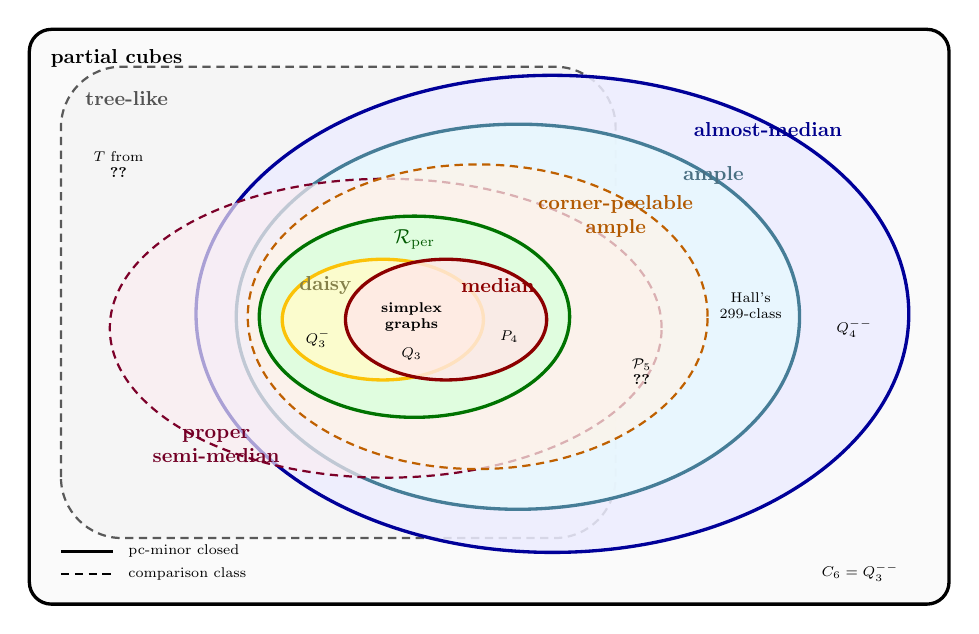
\begin{tikzpicture}[
  scale=.73,
  every node/.style={transform shape},
  stable/.style={very thick},
  contextual/.style={thick,densely dashed},
  witness/.style={font=\scriptsize,inner sep=1pt}
]
  \fill[gray!4,rounded corners=8pt] (0,0) rectangle (16,10);
  \draw[stable,rounded corners=8pt] (0,0) rectangle (16,10);
  \node[anchor=north west,font=\bfseries] at (.25,9.78)
    {partial cubes};

  % The dashed outer comparison classes have no asserted pairwise relation
  % beyond the displayed containments.
  \fill[gray!8,rounded corners=22pt] (.55,1.15) rectangle (10.2,9.35);
  \draw[contextual,gray!70!black,rounded corners=22pt]
    (.55,1.15) rectangle (10.2,9.35);
  \node[anchor=north west,font=\bfseries,gray!65!black] at (.85,9.05)
    {tree-like};

  \fill[blue!7,opacity=.85] (9.1,5.05) ellipse (6.2 and 4.15);
  \draw[stable,blue!60!black] (9.1,5.05) ellipse (6.2 and 4.15);
  \node[font=\bfseries,blue!55!black] at (12.85,8.25)
    {almost-median};

  \fill[cyan!9,opacity=.85] (8.5,5.0) ellipse (4.9 and 3.35);
  \draw[stable,cyan!55!black] (8.5,5.0) ellipse (4.9 and 3.35);
  \node[font=\bfseries,cyan!45!black] at (11.9,7.45) {ample};

  \fill[purple!7,opacity=.68] (6.2,4.8) ellipse (4.8 and 2.6);
  \draw[contextual,purple!65!black] (6.2,4.8) ellipse (4.8 and 2.6);
  \node[font=\bfseries,purple!60!black,align=center] at (3.25,2.75)
    {proper\\semi-median};

  \fill[orange!9,opacity=.72] (7.8,5.0) ellipse (4.0 and 2.65);
  \draw[contextual,orange!75!black] (7.8,5.0) ellipse (4.0 and 2.65);
  \node[font=\bfseries,orange!70!black,align=center] at (10.2,6.75)
    {corner-peelable\\ample};

  \fill[green!13,opacity=.92] (6.7,5.0) ellipse (2.7 and 1.75);
  \draw[stable,green!45!black] (6.7,5.0) ellipse (2.7 and 1.75);
  \node[font=\bfseries,green!35!black] at (6.7,6.35) {\(\Rper\)};

  \fill[yellow!20,opacity=.9] (6.15,4.95) ellipse (1.75 and 1.05);
  \draw[stable,yellow!55!orange] (6.15,4.95) ellipse (1.75 and 1.05);
  \fill[red!9,opacity=.82] (7.25,4.95) ellipse (1.75 and 1.05);
  \draw[stable,red!55!black] (7.25,4.95) ellipse (1.75 and 1.05);

  \node[font=\bfseries,yellow!45!black] at (5.15,5.55) {daisy};
  \node[font=\bfseries,red!55!black] at (8.15,5.55) {median};
  \node[font=\scriptsize\bfseries,align=center] at (6.65,5.0)
    {simplex\\graphs};

  \node[witness] at (5.02,4.62) {\(Q_3^-\)};
  \node[witness] at (8.35,4.65) {\(P_4\)};
  \node[witness] at (6.65,4.35) {\(Q_3\)};
  \node[witness,align=center] at (1.55,7.65)
    {\(T\) from\\\cref{ex:tree-like-not-recursive}};
  \node[witness,align=center] at (10.65,4.05)
    {\(\mathcal P_5\)\\\cref{prop:pentagonal}};
  \node[witness,align=center] at (12.55,5.2)
    {Hall's\\299-class};
  \node[witness] at (14.35,4.8) {\(Q_4^{--}\)};
  \node[witness] at (14.45,.55) {\(C_6=Q_3^{--}\)};

  \draw[stable] (.55,.92)--(1.45,.92);
  \node[anchor=west,font=\scriptsize] at (1.6,.92) {pc-minor closed};
  \draw[contextual] (.55,.52)--(1.45,.52);
  \node[anchor=west,font=\scriptsize] at (1.6,.52) {comparison class};
\end{tikzpicture}
\caption{Venn-style containment diagram for the classes used in the paper.
Solid outlines mark pc-minor-closed classes; dashed outlines mark comparison
classes for which no pc-minor-closure assertion is made here.  Complete
enclosure records a proved containment.  Intersections of nonnested outer
outlines are schematic and assert no further relationship.  The labels
\(T\) and \(\mathcal P_5\) witness the strict containments of \(\Rper\) in
the indicated outer comparison classes.  Hall's maximum class and
\(Q_4^{--}\) witness the two strict containments in the surrounding
corner-peelable--ample--almost-median chain.}
\label{fig:class-position}
\end{figure}

\section{Closure properties and inherited consequences}
\label{sec:closure}

The hereditary characterizations already give pc-minor, convex-subgraph,
and gated-subgraph closure.  The following proposition records the remaining
elementary operations and the exact limitations.

\begin{proposition}[Elementary closure properties]
\label{prop:closure}
For finite partial cubes, the following statements hold.
\begin{enumerate}[label=\textup{(\roman*)}]
  \item A specified peripheral expansion of \(B\) along an isometric site
        \(S\) belongs to \(\Rper\) if and only if both \(B\) and \(S\) do.
  \item \(G\square H\in\Rper\) if and only if \(G,H\in\Rper\).
  \item \(\Rper\) is closed under convex and gated subgraphs, but not under
        arbitrary isometric or arbitrary induced subgraphs.
\end{enumerate}
\end{proposition}

\begin{proof}
For (i), necessity follows because \(B\) is a contraction and \(S\) is a
semicube restriction of the output; sufficiency is the defining closure
rule.

For (ii), use induction on \(\idim(G)+\idim(H)\).  If \(G\) is the
peripheral expansion of \(B\) along \(S\), then \(G\square H\) is the
peripheral expansion of \(B\square H\) along \(S\square H\), and both
smaller products recursively qualify.  The base case is a singleton factor,
for which the product is the other factor; if only \(H\) is nontrivial, swap
the factors.  Conversely, each factor is a convex layer of the product and
hence belongs to \(\Rper\) by \cref{lem:pcminor-closure}.

Convex and gated closure in (iii) follows from
\cref{lem:pcminor-closure}.  For the negative assertions, the hypercube
\(Q_3\) is median and hence belongs to \(\Rper\), but
the middle-level \(C_6=Q_3^{--}\) is an induced isometric subgraph and is
periphery-free.
\end{proof}

\begin{remark}[What heredity is and is not obtained]
The valid chain for subgraphs of a fixed graph is
\[
 \text{gated}\Longrightarrow\text{convex}
 \Longrightarrow\text{isometric}\Longrightarrow\text{induced}.
\]
\Cref{lem:pcminor-closure} gives convex-subgraph closure and therefore also
gated-subgraph closure.  It does not give closure under the two weaker
notions, as \cref{prop:closure}(iii) shows.  This differs from the standard
tree-like class, for which gated-subgraph closure is valid but
convex-subgraph closure fails \cite{Gologranc14treehamming}.
\end{remark}

Several further properties follow from known results for the tree-like or
ample classes. The \emph{cubical complex} of a coordinate family is formed
by filling every contained cube, including all its faces. An elementary
cubical collapse removes a maximal cube together with a facet contained in
no other maximal cube. A complex is \emph{collapsible} if a sequence of such
collapses leaves one vertex.

The intersection graph of the maximal cubes has those cubes as vertices,
with adjacency when they meet. For this graph, \emph{dismantlable} means
reducible to one vertex by repeatedly deleting a vertex \(u\) whose closed
neighborhood is contained in that of another vertex \(v\). This is the
graph-theoretic meaning of dismantlability, distinct from a corner peeling
of the original partial cube.

\Needspace{10\baselineskip}
\begin{proposition}[Inherited structural properties]
\label{prop:inherited-properties}
Let \(G\in\Rper\).  Then:
\begin{enumerate}[label=\textup{(\roman*)}]
  \item if \(G\) is regular, then \(G\) is a hypercube;
  \item the intersection graph of the maximal cubes of \(G\) is
        dismantlable;
  \item if \(\alpha_i(G)\) is the number of induced \(i\)-cubes, then
        \(\sum_{i\ge0}(-1)^i\alpha_i(G)=1\); and
  \item the cubical complex of \(G\) is collapsible, and hence contractible.
\end{enumerate}
\end{proposition}

\begin{proof}
The first three conclusions hold for every tree-like partial cube
\cite{BresarImrichKlavzar03}; the corrected proof of (ii) is
\cite[Corollary~15]{Gologranc14treehamming}.  They therefore follow from
\cref{prop:position}(ii). The specialization of (i) to convex-treelike
graphs is also \cite[Proposition~5.9]{Polat12treelike}.
For (iv), ampleness from \cref{prop:position}(ii) suffices:
the cubical complex of every ample class is collapsible
\cite[Proposition~4.12]{ChalopiChepoiMoran22}. The corner peeling also gives
such a sequence directly, as described in Section~4.4 of that source.
\end{proof}

\begin{remark}[Weak retracts]
Gologranc identified a gap in the original proof of weak-retract closure
for tree-like partial cubes and left that question open in
\cite{Gologranc14treehamming}.  The closure results here concern convex
subgraphs and coordinate quotients.
\end{remark}

\section{Explicit ample obstructions}
\label{sec:obstructions}

The nonample obstruction family was identified in
\cref{prop:punctured-cubes}.  We now give explicit ample members of the
second family in \cref{thm:complete-rper-basis}, beginning with the smallest
one beyond the punctured cubes.

The following table provides a quick gallery before the general two-layer
formalism.  The first three rows are globally ordered: there is no
obstruction of order below six, \(Q_4^{--}\) is the next nonample member, and
\(\mathcal P_5\) is the smallest obstruction outside the punctured-cube
family.  The later rows are small named examples, not a claim that all
intervening orders have been classified.

\begin{center}
\small
\begin{tabular}{@{}c c c p{0.48\textwidth}@{}}
\toprule
Obstruction & Order & \(\idim\) & Description \\
\midrule
\(Q_3^{--}\cong C_6\) & 6 & 3
  & first obstruction; nonample and periphery-free \\
\(Q_4^{--}\) & 14 & 4
  & second antipodally punctured cube; nonample \\
\(\mathcal P_5\) & 16 & 5
  & smallest additional obstruction; maximum of VC dimension two,
    \cref{prop:pentagonal,thm:global-minimality} \\
\(\mathcal A_n\), \(n\ge5\) & \(3n+1\) & \(n\)
  & cyclic arcs of length at most three; infinite ample family with
    \(\mathcal A_5=\mathcal P_5\), \cref{thm:cyclic-arcs} \\
\(\mathcal F_n\), \(n\ge9\) odd & \(10n+1\) & \(n\)
  & VC dimension three; peeled in steps of two,
    \cref{thm:step-two} \\
\(\mathcal S_{18}\) & 18 & 6
  & ample square-amalgam obstruction with no cut vertex,
    \cref{prop:square-amalgam-obstruction} \\
\(\mathcal W_8\) & 21 & 8
  & ample one-vertex amalgam of two root-critical factors,
    \cref{prop:rooted-wedge-obstruction} \\
\(\mathcal H_{22}\) & 22 & 6
  & ample obstruction extracted from Hall's maximum class,
    \cref{prop:hall-obstruction} \\
\bottomrule
\end{tabular}
\end{center}

\subsection{The pentagonal obstruction}

Let \(C_5\) be the cycle on \([5]=\{0,1,2,3,4\}\), with indices modulo five,
and define
\begin{equation}
 \mathcal P_5
  =\{\varnothing\}\cup\binom{[5]}1\cup E(C_5)
      \cup\{[5]\setminus e:e\in E(C_5)\}
  \subseteq2^{[5]}.
 \label{eq:pentagonal}
\end{equation}
Thus \(\mathcal P_5\) has sixteen vertices.

\begin{proposition}[Pentagonal obstruction]
\label{prop:pentagonal}
The graph \(\mathcal P_5\) is a maximum VC-dimension-two ample partial cube,
has a corner peeling, and is proper semi-median.  Moreover,
\[
 \mathcal P_5\in\Oper\setminus\{Q_n^{--}:n\ge3\}.
\]
\end{proposition}

\begin{proof}
Every coordinate pair is shattered.  For an edge of \(C_5\), the two-one
pattern is supplied by that edge; for a nonedge, choose an edge disjoint from
the pair and use its complement.  The empty set and singletons supply the
other three patterns.  No triple \(T\) is shattered.  If \([5]\setminus T\)
is not an edge, no member realizes the all-one pattern on \(T\).  If it is
an edge, the vertices of \(T\) induce a path; the pattern selecting the two
endpoints and omitting the middle vertex is absent.  Hence
\[
 \dim_{\mathrm{VC}}(\mathcal P_5)=2,\qquad
 |\mathcal P_5|=1+5+\binom52.
\]
The family is maximum, hence ample and a partial cube.  Every ample class of
VC dimension at most two has a corner peeling
\cite[Proposition~4.11]{ChalopiChepoiMoran22}.

For every coordinate, the projected sections have orders ten and six, their
intersection has order five, and neither contains the other.  By cyclic
symmetry, take coordinate \(0\): the singleton \(\{2\}\) occurs only in the
zero-section, whereas the nonedge \(\{1,4\}\) occurs only in the one-section.
Thus every coordinate is nonperipheral and
\(\mathcal P_5\notin\Rper\).

It remains to verify pc-minimality.  Cyclic symmetry leaves three types of
elementary minor: the two restrictions, of orders six and ten, and the
contraction, of order eleven.  Up to cube symmetry their vertex families are
\begin{align*}
 H_6={}&\{0000,0001,0010,0011,0111,1000\},\\
 H_{10}={}&\{0000,0001,0010,0011,0101,0110,0111,1000,1001,1010\},\\
 H_{11}={}&\{0000,0001,0010,0011,0100,0110,0111,1000,1001,1011,1100\}.
\end{align*}
\Cref{app:finite-decompositions} gives an explicit recursive decomposition
of each of these three families.  Thus all fifteen elementary pc-minors
belong to \(\Rper\).  By
\cref{lem:pcminor-closure}, so does every proper pc-minor, and
\(\mathcal P_5\in\Oper\).

Finally, in each coordinate the overlap of the two sections is a
five-vertex path.  Both sections and their contraction belong to \(\Rper\)
by the decompositions in \cref{app:finite-decompositions} and hence are
proper semi-median by
\cref{prop:position}.  The output \(\mathcal P_5\) is ample and therefore
almost-median, hence semi-median.  Its connected expansion across any
coordinate satisfies the recursive definition of proper semi-median
\cite[Section~3, class~(10)]{journals/jgt/BresarIKMS02}.
\end{proof}

\begin{corollary}[Sharpness of the position statements]
\label{cor:position-sharp}
The containments
\[
 \Rper\subsetneq
 \{\text{tree-like}\}\cap\{\text{proper semi-median}\}
\]
and
\[
 \Rper\subsetneq
 \{\text{tree-like}\}\cap\{\text{almost-median}\}
 \cap\{\text{ample and corner-peelable}\}
\]
are strict.
\end{corollary}

\begin{proof}
Form the peripheral expansion
\[
 X=(Q_5\times\{0\})\cup(\mathcal P_5\times\{1\}).
\]
It is tree-like.  The overlap \(\mathcal P_5\) is isometric, and the two
cover members \(Q_5,\mathcal P_5\) are almost-median, so the one-step
preservation theorem makes \(X\) almost-median
\cite[Theorem~4]{BresarImrichKlavzar03fast}.  The same cover witnesses that
\(X\) is proper semi-median: both members are recursively proper
semi-median, the overlap is connected, and the output is semi-median.

The shattering calculation in the proof of \cref{prop:position} shows that a
peripheral expansion of an ample base along an ample isometric site is
ample.  The concatenated prefix-isometric ordering there gives a corner
peeling.  However, \(\mathcal P_5\times\{1\}\) is a convex semicube of
\(X\).  If \(X\in\Rper\), convex-subgraph closure would put
\(\mathcal P_5\) in \(\Rper\), a contradiction.
\end{proof}

\subsection{An infinite family of cyclic-arc obstructions}

The pentagonal class has a second description.  Index the coordinates by
\(\mathbb Z_5\).  An edge \(\{i,i+1\}\) of \(C_5\) is a cyclic arc of length
two, and its complement is the cyclic arc \(\{i+2,i+3,i+4\}\) of length three.
Thus \(\mathcal P_5\) consists of the empty set and all cyclic arcs of length
at most three.  Keeping the arc length fixed while the cycle grows gives an
infinite family of ample obstructions.

For \(n\ge4\) and \(a\in\mathbb Z_n\), write
\([a,a+\ell)=\{a,a+1,\ldots,a+\ell-1\}\subseteq\mathbb Z_n\) for the
cyclic arc of length \(\ell\), and put
\begin{equation}
 \mathcal A_n=\{\varnothing\}\cup
 \{[a,a+\ell):a\in\mathbb Z_n,\ 1\le\ell\le3\}
 \subseteq2^{\mathbb Z_n}.
 \label{eq:cyclic-arcs}
\end{equation}
The \(3n\) arcs are distinct, so \(|\mathcal A_n|=3n+1\), and
\(\mathcal A_5=\mathcal P_5\).  For the proof we also use the path-interval
families
\begin{equation}
 \mathcal J_m=\{\varnothing\}\cup
 \{\{a,\ldots,a+\ell-1\}:1\le a,\ a+\ell-1\le m,\ 1\le\ell\le3\}
 \subseteq2^{[m]},\qquad m\ge0.
 \label{eq:path-intervals}
\end{equation}

\begin{lemma}[Path intervals]
\label{lem:path-intervals}
Every \(\mathcal J_m\) belongs to \(\Rper\).
\end{lemma}

\begin{proof}
Induct on \(m\); \(\mathcal J_0=\{\varnothing\}\) is a singleton.  For
\(m\ge1\), the members of \(\mathcal J_m\) containing \(m\) are
\(\{m\},\{m-1,m\},\{m-2,m-1,m\}\), as far as these are defined.  Deleting
\(m\) gives \(\varnothing,\{m-1\},\{m-2,m-1\}\), which are members of
\(\mathcal J_m\) avoiding \(m\).  Hence the \(1\)-semicube of coordinate
\(m\) is peripheral.  Its contraction base is the zero section
\(\mathcal J_{m-1}\), and its duplicated site is a path with at most three
vertices.  The base lies in \(\Rper\) by induction, and the site is a tree
and hence lies in \(\Rper\) by \cref{prop:position}.
\end{proof}

\begin{theorem}[Cyclic-arc obstructions]
\label{thm:cyclic-arcs}
For every \(n\ge5\), the family \(\mathcal A_n\) is an ample partial cube of
VC dimension two and isometric dimension \(n\) with \(3n+1\) vertices, and
\[
 \mathcal A_n\in\Oper\setminus\{Q_m^{--}:m\ge3\}.
\]
\end{theorem}

\begin{proof}
\emph{Shattering.}  The empty set and the singletons supply the patterns
\(00,10,01\) on every pair \(\{i,j\}\).  The pattern \(11\) is realized
exactly when some arc of length at most three contains both points, that is,
when their cyclic distance is one or two.  Hence
\(\strc(\mathcal A_n)\) contains exactly \(2n\) pairs.  No triple is
shattered.  A triple with the pattern \(111\) lies in an arc of length three,
so it is \(\{i,i+1,i+2\}\).  An arc containing \(i\) and \(i+2\) but not
\(i+1\) runs the other way around the cycle and has length at least
\(n-1\ge4\).  Therefore
\[
 |\strc(\mathcal A_n)|=1+n+2n=|\mathcal A_n|,
\]
and \(\mathcal A_n\) has VC dimension two.  Every shattered set is strongly
shattered: \(\{i\}\) by the edge from \(\varnothing\) to \(\{i\}\);
\(\{i,i+1\}\) by the square
\(\varnothing,\{i\},\{i+1\},\{i,i+1\}\); and \(\{i,i+2\}\) by the square
\(\{i+1\},\{i,i+1\},\{i+1,i+2\},\{i,i+1,i+2\}\).  Thus
\(\mathcal A_n\) is ample \cite{BandeltCDK06}.  Ample families induce
isometric subgraphs of the cube \cite{BandeltCDK06}, so
\(\mathcal A_n\) is a partial cube.  Every coordinate is nonconstant, so its
isometric dimension is \(n\).

\emph{No peripheral coordinate.}  Rotation acts transitively on the
coordinates, so consider coordinate \(0\).  Its projected sections are
\[
 S^1=\{x\setminus\{0\}:0\in x\in\mathcal A_n\},\qquad
 S^0=\{x\in\mathcal A_n:0\notin x\}.
\]
Since \(n\ge5\), the singleton \(\{3\}\) lies in \(S^0\) but not in \(S^1\),
whereas \(\{n-1,1\}=[n-1,n+2)\setminus\{0\}\) lies in \(S^1\) but is not an
arc avoiding \(0\).  Neither section contains the other, so
\(\mathcal A_n\) has no peripheral coordinate and
\(\mathcal A_n\notin\Rper\).

\emph{Minimality.}  Again consider coordinate \(0\).  The zero section
\(S^0\) consists of the empty set and the arcs avoiding \(0\).  These are
the intervals of length at most three in the path \(1,2,\ldots,n-1\), so
\(S^0\cong\mathcal J_{n-1}\in\Rper\) by \cref{lem:path-intervals}.

The one section is
\[
 S^1=\{\varnothing,\{1\},\{n-1\},\{1,2\},\{n-2,n-1\},\{n-1,1\}\}.
\]
It is the square on \(\varnothing,\{1\},\{n-1\},\{n-1,1\}\) with pendant
vertices \(\{1,2\}\) and \(\{n-2,n-1\}\); the four active coordinates
\(n-2,n-1,1,2\) are distinct because \(n\ge5\).  The \(1\)-semicube of
coordinate \(2\) is the single vertex \(\{1,2\}\), whose neighbor \(\{1\}\)
is present.  It is therefore peripheral, with a singleton site.  Removing it,
and then removing \(\{n-2,n-1\}\) in the same way, leaves a square.  Thus
\(S^1\in\Rper\).

The contraction \(K=\mathcal A_n/0\) consists of the empty set, the arcs
avoiding \(0\), and the sets
\[
 \varnothing,\ \{1\},\ \{n-1\},\ \{1,2\},\ \{n-2,n-1\},\ \{n-1,1\}
\]
obtained by deleting \(0\) from arcs through it.  All of these except
\(\{n-1,1\}\) already avoid \(0\).  In \(K\), consider coordinate \(1\).
The members containing \(1\) are \(\{1\},\{1,2\},\{1,2,3\},\{n-1,1\}\).
Deleting \(1\) gives \(\varnothing,\{2\},\{2,3\},\{n-1\}\), and these are
members of \(K\) avoiding \(1\).  Hence the \(1\)-semicube of coordinate
\(1\) is peripheral.  Its duplicated site is the path
\(\{n-1\},\varnothing,\{2\},\{2,3\}\), which lies in \(\Rper\).  Its
contraction base consists of the members of \(K\) avoiding \(1\).  These
are the intervals of length at most three in the path
\(2,3,\ldots,n-1\), together with the empty set, so the base is isomorphic
to \(\mathcal J_{n-2}\in\Rper\).  Thus \(K\in\Rper\).

By rotation, every elementary restriction and contraction of
\(\mathcal A_n\) belongs to \(\Rper\).  \Cref{lem:pcminor-closure} puts
every proper pc-minor in \(\Rper\), so \(\mathcal A_n\in\Oper\).  Since
\(\mathcal A_n\) is ample, it is not a punctured cube \(Q_m^{--}\).
\end{proof}

\begin{remark}[Why the arc length is three]
\label{rem:arc-length}
With arcs of length at most two, the family is a daisy cube: it is a
down-set in \(2^{\mathbb Z_n}\).  It therefore lies in \(\Rper\) by
\cref{prop:position}.  With arcs of length at most four, the family is not a
partial cube for \(n\le6\).  For \(n\ge7\) its contraction is the family of
arcs of length at most four on \(\mathbb Z_{n-1}\), with the three arcs of
length four through one edge missing.  An exact check for
\(7\le n\le9\) finds this contraction outside \(\Rper\).  The maximum
classes of VC dimension two formed by the empty set and all cyclic arcs of
length at most \((n+1)/2\), for odd \(n\), agree with \(\mathcal P_5\) at
\(n=5\).  They are not obstructions for \(n=7,9\).  Thus the fixed length
three is exactly what makes the pentagonal obstruction extend to all
\(n\ge5\).  The same check confirms \cref{thm:cyclic-arcs} directly for
\(5\le n\le13\).
\end{remark}

\subsection{A family of VC dimension three peeled in steps of two}

The second family has VC dimension three and exists exactly on cycles of
odd length in the range we tested. Its proof shows how the parity enters:
the recursive peeling of a minor advances around \(\mathbb Z_n\) in steps
of two, and it reaches every coordinate only when \(2\) generates
\(\mathbb Z_n\).

For \(n\ge9\), call a nonempty set \(S\subseteq\mathbb Z_n\)
\begin{itemize}[leftmargin=2em]
  \item \emph{short} if \(|S|\le3\) and \(S\subseteq[a,a+4)\) for some
        \(a\);
  \item \emph{long} if \(\{a,a+2,a+4\}\subseteq S\subseteq[a,a+5)\) and
        \(|S|\le4\) for some \(a\), called its \emph{left end}; then
        \(a+2\) is its \emph{midpoint}.
\end{itemize}
Put
\begin{equation}
 \mathcal F_n=\{\varnothing\}\cup\{S:S\text{ short or long}\}
 \subseteq2^{\mathbb Z_n}.
 \label{eq:step-two-family}
\end{equation}
Up to translation, the nonempty members are
\[
 \{0\},\ \{0,1\},\ \{0,2\},\ \{0,3\},\ \{0,1,2\},\ \{0,1,3\},\ \{0,2,3\},\
 \{0,2,4\},\ \{0,1,2,4\},\ \{0,2,3,4\}.
\]
Since \(n\ge9\), every nonempty member lies in an arc of length at most
five, and this arc is unique; hence these ten types give
\(10n\) distinct members and \(|\mathcal F_n|=10n+1\).  Equivalently,
\(\mathcal F_n\) is the union of \(\{\varnothing\}\) with the dihedral
orbits of \(\{0\},\{0,1\},\{0,2\},\{0,3\},\{0,1,2\},\{0,1,3\},
\{0,2,4\},\{0,1,2,4\}\).

\begin{lemma}[Deleting one point]
\label{lem:step-two-deletion}
Let \(n\ge9\), let \(S\in\mathcal F_n\), and let \(x\in S\).  Then
\(S\setminus\{x\}\in\mathcal F_n\), unless \(S\) is long with midpoint
\(x\).  In the exceptional case \(S\setminus\{x\}\notin\mathcal F_n\).
\end{lemma}

\begin{proof}
A nonempty subset of a short set is short.  Let \(S\) be long with left end
\(a\).  Deleting \(a+1\) or \(a+3\) leaves the long set
\(\{a,a+2,a+4\}\).  Deleting \(a\) leaves at most three points of
\([a+1,a+5)\), a short set, and deleting \(a+4\) is symmetric.  If
\(x=a+2\), then \(S\setminus\{x\}\) contains \(a\) and \(a+4\) but not
\(a+2\).  Its unique arc of length at most five is \([a,a+5)\), so it is
neither short nor long.
\end{proof}

\begin{theorem}[Step-two obstructions]
\label{thm:step-two}
For every odd \(n\ge9\), the family \(\mathcal F_n\) is an ample partial cube
of VC dimension three and isometric dimension \(n\) with \(10n+1\)
vertices, and
\[
 \mathcal F_n\in\Oper\setminus\{Q_m^{--}:m\ge3\}.
\]
In every coordinate one of the two one-sided section defects has exactly
three vertices, and these three vertices induce a path.
\end{theorem}

The proof has three steps.  Ampleness is a count of shattered sets.  For
minimality it suffices, by rotation, to treat coordinate \(0\).  Its
one-section is a fixed \(27\)-vertex family \(L\).  Its zero-section and
its contraction are peeled one coordinate at a time along
\(2,4,6,\ldots\); \cref{lem:step-two-deletion} makes each of these
coordinates peripheral, and every duplicated site is a pc-minor of \(L\).

\begin{proof}
\emph{Shattering.}  If \(\mathcal F_n\) shatters \(T\), then \(T\) is
contained in a member.  Up to translation and reflection, the subsets of
members with at least two points are the pairs \(\{0,d\}\), \(1\le d\le4\),
the triples
\[
 \{0,1,2\},\ \{0,1,3\},\ \{0,1,4\},\ \{0,2,4\},
\]
and the two long quadruples.  The triple \(\{i,i+2,i+4\}\) is not
shattered: a member containing \(i\) and \(i+4\) is long with left end
\(i\), and therefore contains \(i+2\).  Consequently neither long
quadruple is shattered.  Every other listed set is strongly shattered.
The pairs \(\{i,i+d\}\) with \(d\le3\) and the triples
\(\{i,i+1,i+2\}\), \(\{i,i+1,i+3\}\), \(\{i,i+2,i+3\}\) have all their
subsets short, so they span a cube at \(\varnothing\).  The sets
\(\{i,i+4\}\), \(\{i,i+1,i+4\}\), and \(\{i,i+3,i+4\}\) span cubes at
\(\{i+2\}\): each union of \(\{i+2\}\) with one of their subsets is short
or long.  Counting the empty set, singletons, \(4n\) pairs, and \(5n\)
triples gives
\[
 |\sstrc(\mathcal F_n)|=|\strc(\mathcal F_n)|=1+n+4n+5n=|\mathcal F_n|.
\]
Hence \(\mathcal F_n\) is ample of VC dimension three
\cite{BandeltCDK06}, and in particular it is a partial cube.  All \(n\)
coordinates are nonconstant.

\emph{No peripheral coordinate.}  Rotations are automorphisms, so consider
coordinate \(0\), with sections
\[
 S^1=\{U:U\cup\{0\}\in\mathcal F_n,\ 0\notin U\},\qquad
 S^0=\{U\in\mathcal F_n:0\notin U\}.
\]
By \cref{lem:step-two-deletion},
\[
 S^1\setminus S^0=\{\{-2,2\},\{-2,-1,2\},\{-2,1,2\}\},
\]
the three long sets with midpoint \(0\) after deleting \(0\).  They induce
the path
\[
 \{-2,-1,2\},\ \{-2,2\},\ \{-2,1,2\}.
\]  In the other direction,
\(\{5\}\in S^0\), whereas \(\{0,5\}\) is not a member: a two-point member is
short, so its points have cyclic distance at most three.  Thus
coordinate \(0\) is not peripheral, and \(\mathcal F_n\notin\Rper\).

\emph{The one-section.}  The family \(L=S^1\) depends only on the arc
\([-4,5)\), whose nine points are distinct.  Its \(27\) members are the
empty set, the six singletons \(\{\pm1\},\{\pm2\},\{\pm3\}\), the nine
short pairs
\[
 \{-3,-2\},\{-3,-1\},\{-2,-1\},\{-2,1\},\{-1,1\},\{-1,2\},\{1,2\},\{1,3\},
 \{2,3\},
\]
and the eleven sets coming from long members through \(0\):
\[
\begin{gathered}
 \{2,4\},\{1,2,4\},\{2,3,4\},\ \{-4,-2\},\{-4,-3,-2\},\{-4,-2,-1\},\\
 \{-2,2\},\{-2,-1,2\},\{-2,1,2\},\ \{-1,1,3\},\{-3,-1,1\}.
\end{gathered}
\]
The members containing \(4\) are \(\{2,4\},\{1,2,4\},\{2,3,4\}\); deleting
\(4\) gives members, so the \(1\)-semicube of \(4\) is peripheral with a
three-vertex path as site.  The coordinate \(-4\) is symmetric.  In the
remaining family, the members containing \(3\) are
\[
 \{3\},\ \{1,3\},\ \{2,3\},\ \{-1,1,3\};
\]
deleting \(3\) gives the tree \(\varnothing,\{1\},\{2\},\{-1,1\}\),
all of whose vertices remain.  The
coordinate \(-3\) is symmetric.  In the \(13\)-member family left on
\(\{-2,-1,1,2\}\), the members containing \(2\) are
\[
 \{2\},\ \{-1,2\},\ \{1,2\},\ \{-2,2\},\ \{-2,-1,2\},\ \{-2,1,2\}.
\]
Deleting \(2\) gives
\[
 \{\varnothing,\{-2\}\}\times\{\varnothing,\{-1\},\{1\}\},
\]
a median graph, and all six vertices remain.  What is left is
\(2^{\{-2,-1,1\}}\setminus\{\{-2,-1,1\}\}\), a cube with one vertex
deleted, which belongs to \(\Rper\) by the proof of
\cref{prop:punctured-cubes}.  Trees and median graphs belong to \(\Rper\)
by \cref{prop:position}.  Each displayed peripheral step reconstructs the
previous family, so \(L\in\Rper\).  By rotation, the one-section
\(L_p=\{U:U\cup\{p\}\in\mathcal F_n,\ p\notin U\}\) at every coordinate
\(p\) is isomorphic to \(L\).

\emph{Peeling in steps of two.}  For \(Z\subseteq\mathbb Z_n\) and an
optional point \(c\notin Z\), put
\[
 H(Z;c)=\{S\setminus\{c\}:S\in\mathcal F_n,\ S\cap Z=\varnothing\},
\]
and write \(H(Z)\) when no point is contracted.  These are pc-minors of
\(\mathcal F_n\): restrict every coordinate of \(Z\) to zero and contract
\(c\).  They are therefore partial cubes.

\emph{Claim.}  Let \(p\notin Z\cup\{c\}\) and \(p-2\in Z\cup\{c\}\).  Then
in \(H=H(Z;c)\) the \(1\)-semicube of \(p\) is peripheral.  Its zero-section
is \(H(Z\cup\{p\};c)\), and its duplicated site lies in \(\Rper\).

Let \(T\in H\) contain \(p\), say \(T=S\setminus\{c\}\) with
\(S\in\mathcal F_n\) avoiding \(Z\).  If \(S\setminus\{p\}\in\mathcal F_n\),
then \(T\setminus\{p\}=(S\setminus\{p\})\setminus\{c\}\in H\).  Otherwise,
by \cref{lem:step-two-deletion}, \(S\) is long with midpoint \(p\), so
\(p-2\in S\).  As \(S\) avoids \(Z\), this forces \(p-2=c\).  Then
\(T\setminus\{p\}\) is \(\{p+2\}\), \(\{p-1,p+2\}\), or
\(\{p+1,p+2\}\).  Each is a short member of \(\mathcal F_n\) avoiding
\(Z\cup\{c\}\), so it lies in \(H\).  Thus the one-section of \(p\) is
contained in its zero-section, which proves peripherality.  The
zero-section is \(H(Z\cup\{p\};c)\) by definition.  The duplicated site is
\[
 \{S\setminus\{c,p\}:p\in S\in\mathcal F_n,\ S\cap Z=\varnothing\},
\]
obtained from \(L_p\) by restricting the coordinates in \(Z\) to zero and
contracting \(c\).  It is a pc-minor of \(L_p\cong L\), so it lies in
\(\Rper\) by \cref{lem:pcminor-closure}.  Also \(\{p\}\in H\), so the
coordinate is nonconstant.  This proves the claim.

Because \(n\) is odd, the points \(0,2,4,\ldots,2(n-1)\) are all distinct.
For the zero-section \(S^0=H(\{0\})\), put
\[
 Z_t=\{0,2,\ldots,2t-2\},\qquad p_t=2t\qquad(1\le t\le n-1).
\]
Then \(p_t\notin Z_t\) and \(p_t-2\in Z_t\).  The claim writes
\(H(Z_t)\) as a peripheral expansion of \(H(Z_{t+1})\) along a site in
\(\Rper\).  Since \(Z_n=\mathbb Z_n\), the last family \(H(Z_n)\) is the
singleton \(\{\varnothing\}\).  Descending induction on \(t\) gives
\(S^0=H(Z_1)\in\Rper\).

For the contraction \(\mathcal F_n/0=H(\varnothing;0)\), put \(c=0\) and
\[
 Z_t'=\{2,4,\ldots,2t\},\qquad p_t'=2t+2\qquad(0\le t\le n-2).
\]
Then \(p_t'\notin Z_t'\cup\{0\}\), and \(p_t'-2\) is \(c\) for \(t=0\) and
lies in \(Z_t'\) otherwise.  The claim again gives a chain of peripheral
expansions.  It ends at \(Z_{n-1}'=\mathbb Z_n\setminus\{0\}\), where
\(H(Z_{n-1}';0)=\{\varnothing\}\).  Hence \(\mathcal F_n/0\in\Rper\).

Thus both restrictions and the contraction at \(0\), and by rotation at every
coordinate, belong to \(\Rper\).  \Cref{lem:pcminor-closure} gives
\(\mathcal F_n\in\Oper\).  It is ample, hence not a punctured cube.
Finally, the defect \(S^1\setminus S^0\) computed above has three
vertices inducing a path, and rotation transports this to every
coordinate.  The opposite defect \(S^0\setminus S^1\) is larger: it contains
\(\{5\}\), and \(|S^0|-|S^1\cap S^0|=10n+1-27-24\ge40\).
\end{proof}

\begin{remark}[Parity and verification]
\label{rem:step-two-parity}
The proof uses oddness only to make the step-two walks visit every point.
For even \(n\) they stop after the even coordinates.  An exact check for
\(n=10,12,14\) finds that \(S^0\) and \(\mathcal F_n/0\) are then outside
\(\Rper\), so \(\mathcal F_n\) is not an obstruction.  For odd
\(9\le n\le51\), a program replays every step of both chains, including
each containment and each site.  Independently, the full pc-minor recursion
confirms \(\mathcal F_n\in\Oper\) for \(n=9,11,13,15,17\).  The
coordinate-state test of \cref{thm:coordinate-state-basis} confirms it for
\(n=9\).  \Cref{thm:step-two} also shows that single-vertex deletion from a
member of \(\Rper\) does not produce every ample obstruction.  Here, in
every coordinate, the smaller one-sided defect has three vertices.
\end{remark}

\subsection{No criterion of bounded depth}
\label{sec:no-bounded-depth}

By \cref{thm:coordinate-state-basis}, a periphery-free partial cube is an
obstruction exactly when every proper nontrivial pc-minor, at every depth,
has a peripheral coordinate.  The following family shows that no fixed
depth suffices.  Fix the coordinate \(0\) of \(\mathcal P_5\) and its two
arcs
\[
 a_0=\{1,2,3\},\qquad b_0=\{0,1,2\}.
\]
Each lies in a unique maximal square of \(\mathcal P_5\), namely
\[
 \{2\},\{1,2\},\{2,3\},\{1,2,3\}
 \qquad\text{and}\qquad
 \{1\},\{0,1\},\{1,2\},\{0,1,2\},
\]
and \(a_0\) does not lie in the square of \(b_0\).  For \(k\ge1\), let
\(Y\) be a set of \(k\) new coordinates and put
\begin{equation}
 \mathcal T_k=(\mathcal P_5\times2^Y)\setminus\{(a_0,Y),(b_0,\varnothing)\}.
 \label{eq:puncture-tower}
\end{equation}
The two deleted vertices sit above the antipodal points \(Y\) and
\(\varnothing\) of the auxiliary cube.

\begin{theorem}[No criterion of bounded depth; computer-assisted base]
\label{thm:no-bounded-depth}
For every \(k\ge1\), the family \(\mathcal T_k\) is an ample partial cube of
isometric dimension \(k+5\) with \(2^{k+4}-2\) vertices.  It has no
peripheral coordinate and does not belong to \(\Oper\), since contracting
the \(k\) coordinates of \(Y\) gives \(\mathcal P_5\).  Every nontrivial
pc-minor of \(\mathcal T_k\) obtained by fewer than \(k\) elementary
operations has a peripheral coordinate.
\end{theorem}

Consequently, for every \(d\), the periphery-free partial cubes all of whose
pc-minors of depth less than \(d\) have a peripheral coordinate form a
strictly larger family than \(\Oper\).  The
quantification over all states in \cref{thm:coordinate-state-basis} cannot
be truncated.

\begin{proof}
\emph{Ampleness.}  The product of ample families is ample, since
shattered and strongly shattered sets of a product are the unions of
those of the factors.  In an ample family, a vertex lies in a unique
maximal cube exactly when deleting it leaves an ample family
\cite[Lemma~4.1]{ChalopiChepoiMoran22}.  Maximal cubes of
\(\mathcal P_5\times2^Y\) are products of maximal cubes, so \((a_0,Y)\)
lies only in \(M_a\times2^Y\), where \(M_a\) is the square of \(a_0\).  Its
deletion leaves an ample family.  In that family \((b_0,\varnothing)\) lies
only in \(M_b\times2^Y\), which avoids \((a_0,Y)\) because
\(a_0\notin M_b\).  Deleting it leaves \(\mathcal T_k\) ample.  Ample
families are partial cubes, and every coordinate is nonconstant.

\emph{Fibres.}  For a state \(\tau\) that retains every coordinate of
\(Y\), write \(F=\mathcal P_5[\tau]\), and let \(F^a\) and \(F^b\) be the
corresponding minors of \(\mathcal P_5\setminus\{a_0\}\) and
\(\mathcal P_5\setminus\{b_0\}\).  Then \(\mathcal T_k[\tau]\) has fibre
\(F^a\) over \(Y\), fibre \(F^b\) over \(\varnothing\), and fibre \(F\)
over every other subset of \(Y\).  A coordinate of \(\mathcal P_5\) is
peripheral with a given orientation exactly when the corresponding section
containment holds in each fibre.  An auxiliary coordinate is peripheral
exactly when the fibres on one side are contained in the matching fibres
on the other.  The pairs to compare are \((F^b,F)\) and \((F,F^a)\) when
\(k\ge2\), with further pairs \((F,F)\) when \(k\ge3\).  Hence, for
\(k\ge2\), whether \(\mathcal T_k[\tau]\) has a peripheral coordinate does
not depend on \(k\).  An exact computation of all states \(\tau\) of the
five coordinates of \(\mathcal P_5\), for \(k=1\) and \(k=2\), shows that
\(\mathcal T_k\) itself is periphery-free and that every other state with
at least two vertices has a peripheral coordinate.  There are \(863\) such
states for \(k=1\) and \(917\) for \(k=2\).

\emph{Words touching \(Y\).}  Let a word of fewer than \(k\) elementary
operations apply at least one operation to a coordinate \(s\in Y\).  Then
some \(t\in Y\) is untouched.  Since operations in distinct coordinates
commute, the minor is \(\mathcal T_k[\sigma]\) for a state \(\sigma\).  If
\(s\) is contracted, each deleted vertex is replaced by its
\(s\)-neighbour, which is not the other deleted vertex because \(t\) is
retained.  Thus \(\mathcal T_k[\sigma]=(\mathcal P_5\times2^Y)[\sigma]\) is a
product with a full factor in \(t\), so \(t\) is peripheral.  If \(s\) is
restricted, one deleted vertex lies outside the chosen semicube.  The
minor is then a product in which one fibre may lack a single point, and
the \(t\)-section containing that fibre is contained in the other.  Hence
\(t\) is peripheral, unless the minor has at most two vertices, in which
case it is a vertex or an edge.

\emph{Depth exactly \(k\).}  Words without an operation in \(Y\) are
covered by the fibre computation.  Contracting all of \(Y\) replaces each
deleted vertex by a surviving copy and gives \(\mathcal P_5\), which is
periphery-free and a proper pc-minor.  Therefore
\(\mathcal T_k\notin\Rper\).  It is not minimal, since its proper minor
\(\mathcal P_5\) lies outside \(\Rper\).
\end{proof}

\begin{remark}[Consequences for a generative description]
\label{rem:no-local-generator}
By \cref{prop:deletion-normal-form}, every obstruction is a member of
\(\Rper\) with one defect deleted.  \Cref{thm:no-bounded-depth} limits
what a converse can look like.  Periphery tests at bounded depth cannot
certify minimality, and the family \(\mathcal P_5\times K_2\) shows that
adding \(\Rper\)-membership of the minors along one coordinate is still not
enough.  The criteria in \cref{thm:coordinate-state-basis,sec:repair-recognition}
account for this global minimality condition; a structural generator must
also account for it, although it need not use a recursive membership
predicate.  Unlike daisy membership, a fixed-depth periphery test cannot
supply the condition.

The earlier finite data suggested a defect bound of three vertices, but
this bound is false.  Replacing every coordinate in the signed clauses
of \(\mathcal P_5\) by two coordinates with the same forbidden sign gives
an ample forbidden minor of order \(918\), isometric dimension \(10\),
and VC dimension \(7\), with oriented defects of sizes \(9\) and \(45\)
at every coordinate.  Uniform coordinate-block replacement makes the
minimum defect unbounded even at fixed dimension difference three;
the \href{../minor-atlas/research/coordinate_block_amplification.pdf}{coordinate-block research note}
contains the construction, full proofs, and direct verification.
For one-vertex-decomposable obstructions one vertex suffices in all
\(47\) root-critical factors computed through dimension five; that
separate assertion remains open in general.
\end{remark}

\subsection{The square-amalgam obstruction}

In \(Q_6\), with the leftmost bit denoting coordinate \(5\), define
\begin{equation}
\begin{split}
 \mathcal S_{18}=\{&
 000000,000100,001100,010000,010100,100100,101100,110000,\\
 &110001,110011,110100,111000,111001,111010,111011,111100,
 111110,111111\}.
\end{split}
\label{eq:S18}
\end{equation}

\begin{proposition}[Square-amalgam obstruction; computer-assisted]
\label{prop:square-amalgam-obstruction}
The family \(\mathcal S_{18}\) is an ample VC-dimension-two partial cube and
\[
 \mathcal S_{18}\in\Oper.
\]
It has no cut vertex and is the gated amalgam of two copies of
\(\mathcal L_4\) from \eqref{eq:L4} along a maximal square.  Up to cube
isomorphism, it is the unique ample periphery-free partial cube of isometric
dimension six and order at most eighteen.
\end{proposition}

\begin{proof}
The exact verifier applied to \eqref{eq:S18} checks the Hamming-distance
criterion for a partial cube, Sandwich equality
\[
 |\mathcal S_{18}|=1+6+11,
\]
the absence of a peripheral orientation in every coordinate, and recursive
peripheral expansion trees for all sixteen distinct normalized elementary
pc-minors.  Pc-minor closure then proves
\(\mathcal S_{18}\in\Oper\).  The same computation records a complete
corner peeling, although only ampleness is needed here.

For the amalgam description, put
\[
 A=\{0,1\},\qquad I=\{2,3\},\qquad B=\{4,5\},
\]
and
\[
 L=\{x\in\mathcal S_{18}:x_B=11\},\qquad
 R=\{x\in\mathcal S_{18}:x_A=00\}.
\]
Direct section comparison gives
\[
 \mathcal S_{18}=L\cup R,\qquad
 L\cap R=\{110000,110100,111000,111100\}=11{*}{*}00.
\]
Both \(L\) and \(R\) are eleven-vertex copies of \(\mathcal L_4\), and the
displayed intersection is a maximal square in each.  The Hamming gate of a
vertex is obtained by overwriting the fixed coordinates defining the
corresponding piece; inspection of \eqref{eq:S18} shows that the overwritten
vertex is present.  Hence both pieces are gated.  A direct connectivity check
after deletion of each of the eighteen vertices shows that there is no cut
vertex.

For the bounded uniqueness assertion, the expansion census takes all
\(806\) ample dimension-five bases of order at most seventeen and enumerates
every nonempty intersection and every component assignment outside it.  Of
\(767\,596\) intersections and \(741\,781\) assignments, \(1\,209\) give
periphery-free isometric section pairs.  Exactly three labelled occurrences
are ample, and all three canonicalize to \eqref{eq:S18}.  This proves the
stated uniqueness.
\end{proof}

\subsection{A Hall-derived obstruction}

The maximum VC-dimension-three class of Hall has \(299\) concepts and no
corner \cite[Theorem~4.5]{ChalopiChepoiMoran22}.  A short sequence of
restrictions produces the following additional obstruction.

\Needspace{12\baselineskip}
\begin{proposition}[Hall-derived obstruction; computer-assisted]
\label{prop:hall-obstruction}
The six-coordinate family
\begin{align*}
 \mathcal H_{22}=\{&
 000111,001100,001101,001111,010000,010100,010101,010111,\\
 &011100,011101,011111,101000,101001,101010,101011,101100,\\
 &101101,101111,110000,110100,111000,111100\}
\end{align*}
 is an ample, periphery-free partial cube and is pc-minor-minimal outside
 \(\Rper\).
In particular, \(\mathcal H_{22}\in\Oper\).
\end{proposition}

\begin{proof}
The family is obtained from Hall's \(299\)-concept class by the restrictions
\[
 r^1_{10},r^0_4,r^0_1,r^0_0,r^1_7,r^0_2,
\]
where indices count from the right and are renumbered from zero after each
step. The resulting six-coordinate family is mapped to the displayed one by
\[
 (x_0,x_1,x_2,x_3,x_4,x_5)
 \longmapsto (x_0,x_1,x_2,x_4,1-x_5,1-x_3).
\]
These operations record the provenance of the example but are not used in
its verification. Applied directly to the displayed family, the computation in
\cref{sec:computation} compares its shattering and strong-shattering
complexes, tests both section containments in every coordinate, and checks
every elementary proper pc-minor recursively.  These three checks establish,
respectively, ampleness, absence of a peripheral coordinate, and membership
of every proper pc-minor in \(\Rper\).
\end{proof}

\subsection{The smallest additional obstruction}

The order of a partial cube is constrained by its expansion sites.  The
following elementary lemma closes the high-dimensional part of the
small-order search.

\begin{lemma}[Partial cubes of order at most \(d+2\)]
\label{lem:low-excess}
Let \(G\) be a finite connected partial cube of isometric dimension \(d\).
Then \(|V(G)|\ge d+1\).  Moreover:
\begin{enumerate}[label=\textup{(\roman*)}]
  \item if \(|V(G)|=d+1\), then \(G\) is a tree;
  \item if \(|V(G)|=d+2\), then \(G\) is unicyclic and its unique cycle is
        a square.
\end{enumerate}
In particular, every nontrivial partial cube with
\(|V(G)|\le d+2\) has a peripheral \(\Theta\)-class.
\end{lemma}

\begin{proof}
Reverse a complete sequence of \(d\) \(\Theta\)-class contractions from
\(G\) to \(K_1\), and let \(s_i\) be the number of vertices in the site
duplicated by the \(i\)th reverse expansion.  The new class has one edge for
each vertex of that site, and the expansion adds exactly \(s_i\) vertices.
Hence
\begin{equation}
 |V(G)|=1+\sum_{i=1}^d s_i,\qquad
 |V(G)|-(d+1)=\sum_{i=1}^d(s_i-1).
 \label{eq:expansion-excess}
\end{equation}
Every \(s_i\) is positive, proving the lower bound.

If equality holds, every new \(\Theta\)-class is a singleton.  Such a class
is a one-edge cut and hence a bridge, so reversing the expansions from
\(K_1\) produces a tree.

If \(|V(G)|=d+2\), exactly one duplicated site has order two and all the
others have order one.  Immediately before the exceptional expansion, the
graph is a tree.  The two cover members are isometric subtrees, and their
two-vertex intersection is therefore an edge.  Duplicating it creates one
square and no other cycle.  Each later singleton class is a bridge and
cannot alter the unique cyclic block.  Thus the final graph is a square with
trees attached to its vertices.

A nontrivial tree has a leaf edge, hence a peripheral class.  If trees are
attached to the square, a leaf outside the square again gives one; the bare
square has both coordinates peripheral.
\end{proof}

\begin{theorem}[Global vertex-minimality; computer-assisted]
\label{thm:global-minimality}
The pentagonal graph \(\mathcal P_5\) has the smallest possible isometric
dimension among the members of
\(\Oper\setminus\{Q_n^{--}:n\ge3\}\).  It is the unique additional
obstruction of isometric dimension five and order at most twenty-one.
Moreover, no additional obstruction has fewer than sixteen vertices.
Consequently \(\mathcal P_5\) is vertex-minimal among all additional
obstructions, without a dimension restriction.
\end{theorem}

\begin{proof}
The exact coordinate-isomorphism enumeration through isometric dimension four
contains no additional obstruction.  In dimension five, the exhaustive
expansion enumeration through order twenty-one produces \(14\,259\) partial-cube
representatives, of which \(3\,115\) are periphery-free; the only additional
minimal type is \(\mathcal P_5\).  This proves the first two assertions.

For orders below sixteen, the exact expansion searches in dimensions six
through twelve produce no ample periphery-free partial cube. Every additional
obstruction is ample by \cref{prop:obstruction-structure}, so this is the
required exclusion.  The counts and the
exhaustiveness contract are recorded in \cref{sec:computation}.  If
\(13\le d\le14\) and \(|V(G)|\le15\), then
\(|V(G)|\le d+2\), so \cref{lem:low-excess} supplies a peripheral class.
Finally, a connected partial cube of dimension at least fifteen has at least
\(d+1\ge16\) vertices.  These cases exhaust all dimensions.
\end{proof}

\section{Gated and one-vertex amalgams}
\label{sec:wedges}

One-vertex identifications also occur in Polat's separation of convex-treelike
and faithful-treelike graphs \cite[pp.~69--70]{Polat12treelike}; these
classes are compared in \cref{sec:polat-construction}. Here we
characterize both membership and pc-minor minimality for one-vertex amalgams
by conditions on the pointed factors.

A \emph{gated amalgam} is a union \(G=G_1\cup G_2\) of two intersecting
gated subgraphs.  Call a finite partial cube \emph{gated-prime} if it is not
such a union with both pieces proper.  Minimal obstructions give an exact
reduction of the gated-amalgamation question.

\begin{proposition}[Gated-amalgam reduction]
\label{prop:gated-reduction}
The class \(\Rper\) is closed under gated amalgamation if and only if every
member of \(\Oper\) is gated-prime. Every \(Q_n^{--}\), \(n\ge3\), is
gated-prime.

\emph{Computer-assisted additional assertions.} The examples
\(\mathcal P_5\) and \(\mathcal H_{22}\) are also gated-prime.
\end{proposition}

\begin{proof}
Suppose \(O\in\Oper\) is the gated amalgam of proper subgraphs \(A,B\).
Gated subgraphs are convex, hence \(A,B\) are proper pc-minors of \(O\) and
belong to \(\Rper\).  Closure under gated amalgamation would incorrectly put
\(O\) in the class.

Conversely, assume every member of \(\Oper\) is gated-prime and let
\(G=G_1\cup G_2\) be a gated amalgam with \(G_1,G_2\in\Rper\).  If
\(G\notin\Rper\), take elementary pc-minors
\[
 H_0=G,H_1,\ldots,H_m=O
\]
ending at \(O\in\Oper\).  Track two pieces \(A_k,B_k\), beginning with
\(A_0=G_1,B_0=G_2\).  Under restriction to a nonempty semicube \(W\), put
\(A_{k+1}=A_k\cap W\) and \(B_{k+1}=B_k\cap W\); under contraction
\(\pi_e\), take their images.

Nonempty restrictions of gated pieces remain gated: if \(x,y\in W\) with
\(y\) in the piece, then the gate of \(x\) lies in
\(I(x,y)\subseteq W\).  Contraction images of gated subgraphs are gated by
\cite[Lemma~10]{ChepoiKnauerMarc20}.  At every stage the two images cover
the current graph and are pc-minors of \(G_1,G_2\), so they belong to
\(\Rper\).  Neither image can be empty or the whole current graph, since
then the current graph, and hence its later minor \(O\), would belong to
\(\Rper\).  They continue to intersect: this is immediate under
contraction, while after a restriction disjointness would disconnect the
current semicube because no edge joins the two exclusive parts.  Thus the
final images form a proper gated decomposition of \(O\), contradicting
gated-primality.

For \(Q_n^{--}\), every convex subgraph is the intersection with a Boolean
face.  If one of two proper faces in a putative intersecting cover has
codimension at least two, their union has at most
\[
 2^{n-1}+2^{n-2}-1<2^n-2
\]
vertices.  Otherwise both are halfcubes.  Halfcubes in the same coordinate
are equal or disjoint; in distinct coordinates their union has at most
\(3\cdot2^{n-2}-1<2^n-2\) vertices.  Hence they cannot cover
\(Q_n^{--}\).  For \(\mathcal P_5\) and \(\mathcal H_{22}\), the exact
coordinate-face audit described in \cref{sec:computation} tests all
\(3^5\), respectively \(3^6\), intersections of semicubes, retains the
gated ones, and finds no proper intersecting two-cover.
\end{proof}

The last conclusion does not extend to all obstructions.  To see the exact
failure, we refine the recursion at a distinguished vertex.

\begin{definition}[Root-avoiding decompositions and critical roots]
\label{def:rooted}
A \emph{root-avoiding peripheral decomposition} of a pointed partial cube
\((A,a)\) is defined recursively.  A singleton has such a decomposition.  At
a nontrivial node, the chosen peripheral semicube must omit \(a\); its
duplicated site has an ordinary recursive peripheral decomposition, while the
contraction base, rooted at the image of \(a\), again has a root-avoiding
decomposition.
Let \(\Rbullet\) be the class of pointed partial cubes admitting such a
decomposition.

A nontrivial pointed member \((A,a)\) of \(\Rper\) is \emph{root-locked} if
every peripheral semicube contains \(a\).  It is \emph{root-critical} if it
is root-locked and, for every coordinate \(e\), both the restriction of
\(A\) to the \(e\)-semicube containing \(a\) and the contraction \(A/e\),
with their natural roots, belong to \(\Rbullet\).
\end{definition}

For pointed graphs \((A,a),(B,b)\) on disjoint coordinate sets, write
\(A\vee B\) for their one-vertex amalgam obtained by identifying \(a\) and
\(b\).  Distances between different factors add through the common vertex,
so this amalgam is again a partial cube.

\begin{example}[Why the root matters]
\label{ex:rooted-path}
Root the path \(\{00,10,11\}\) at \(00\). First remove the peripheral
side \(\{11\}\), then the remaining endpoint different from the root.
This is a root-avoiding decomposition. If another partial cube is attached
at \(00\), these same two sides still omit the attachment vertex and can
be removed in the same order. In contrast, attaching a nontrivial graph to
the removed endpoint would enlarge that side and can destroy its
peripherality. The wedge theorem formalizes this distinction; the
eleven-vertex example in \cref{prop:rooted-wedge-obstruction} will show that
a member of \(\Rper\) need not admit root avoidance at every vertex.
\end{example}

\begin{lemma}[Peeling one factor inside a wedge]
\label{lem:rooted-amalgam}
If \((A,a)\in\Rbullet\) and \(B\in\Rper\), then the one-vertex amalgam
obtained by identifying \(a\) with any vertex of \(B\) belongs to \(\Rper\).
\end{lemma}

\begin{proof}
Induct on \(\idim(A)\).  For a singleton, the amalgam is \(B\).  Otherwise
choose the first coordinate in the rooted decomposition.  Its peripheral
semicube omits \(a\), so adjoining \(B\) at \(a\) neither changes that
semicube nor spoils its peripherality.  The contraction is the one-vertex
amalgam of \(B\) with the rooted contraction base of \(A\), and the
duplicated site is unchanged.  The induction hypothesis puts the former in
\(\Rper\), while the decomposition puts the latter there.  The inverse
peripheral expansion proves the claim.
\end{proof}

\begin{theorem}[Rooted-wedge characterization]
\label{thm:rooted-wedge}
Let \((A,a)\) and \((B,b)\) be pointed members of \(\Rper\).
\begin{enumerate}[label=\textup{(\roman*)}]
  \item
  \[
   A\vee B\in\Rper
   \quad\Longleftrightarrow\quad
   (A,a)\in\Rbullet\ \text{or}\ (B,b)\in\Rbullet.
  \]
  \item If \(A,B\) are nontrivial, then \(A\vee B\) is periphery-free if
        and only if both pointed factors are root-locked.
  \item If \(A,B\) are nontrivial, then
  \[
   A\vee B\in\Oper
   \quad\Longleftrightarrow\quad
   (A,a)\ \text{and}\ (B,b)\ \text{are root-critical}.
  \]
\end{enumerate}
Moreover, \(\Rbullet\) is closed under contractions and restrictions to
semicubes containing the root.  Consequently, the root-critical graphs are
exactly the pointed-minor-minimal members of
\[
 \{(A,a):A\in\Rper\}\setminus\Rbullet,
\]
where pointed minors use those two root-preserving operations.
\end{theorem}

The proof uses the same commutation argument as ordinary heredity, with
the additional requirement that the removed side avoid the root. In a
wedge, a coordinate belongs to one factor: the other factor enlarges only
its root side. This identifies the possible peripheral steps and reduces
both membership and minimality to the pointed factors.

\begin{proof}
We first prove closure under root-preserving minors.  Commute one such
operation in coordinate \(f\) past the first coordinate \(e\) of a
root-avoiding decomposition.  If \(f=e\), either contraction or restriction
to the root side leaves the rooted contraction base.  If \(f\ne e\), the
new contraction base and duplicated site are the corresponding \(f\)-minors
of the old ones, and the chosen peripheral side still omits the root.  If
that side becomes empty, or if \(e\) becomes constant, the result is a
root-preserving minor of the old contraction base.  Induction on isometric
dimension, using \cref{lem:pcminor-closure} for the unpointed duplicated
site, proves the asserted closure.

For (i), the reverse implication is \cref{lem:rooted-amalgam} and its
symmetric version.  For necessity, induct on
\(\idim(A)+\idim(B)\).  A singleton factor already lies in \(\Rbullet\), so
assume both are nontrivial and use disjoint coordinate sets.  For a
coordinate \(e\) of \(A\), write \(A_e^a\) and \(A_e^{\bar a}\) for the
projected sections, with the first containing \(a\).  The corresponding
sections of the wedge are
\[
 A_e^a\vee B
 \qquad\text{and}\qquad
 A_e^{\bar a}.
\]
The first contains a vertex of the nontrivial factor \(B\) outside the
\(A\)-coordinate block, so it cannot be contained in the second.
Consequently, \(e\) is peripheral in the wedge exactly when
\(A_e^{\bar a}\subseteq A_e^a\); in that case the peripheral side omits the
root.

Choose the first coordinate of a recursive decomposition of \(A\vee B\),
say it lies in \(A\).  Its contraction base is \(A_e^a\vee B\) and belongs
to \(\Rper\).  By induction, either \((A_e^a,a)\) or \((B,b)\) lies in
\(\Rbullet\).  In the second case we are done.  In the first,
\(A_e^{\bar a}\) is a pc-minor of \(A\) and hence lies in \(\Rper\).
Prepending the peripheral coordinate \(e\) gives a root-avoiding decomposition
for \((A,a)\).  The case in which the first coordinate lies in \(B\) is
symmetric.

The same section calculation proves (ii): a wedge coordinate is peripheral
exactly when its factor has a peripheral semicube avoiding the root.

Suppose both factors are root-critical.  They do not lie in \(\Rbullet\), so
(i) puts their wedge outside \(\Rper\).  For a coordinate \(e\) of \(A\),
restriction to the side omitting the root deletes \(B\) and gives a pc-minor
of \(A\).  Restriction to the root side and contraction give
\[
 A_e^a\vee B
 \qquad\text{and}\qquad
 (A/e)\vee B.
\]
Both lie in \(\Rper\) by (i) and root-criticality.  The same holds for
coordinates of \(B\), so every elementary proper pc-minor of the wedge is
in the class.  Hence \(A\vee B\in\Oper\).

Conversely, let \(A\vee B\in\Oper\).  Every obstruction is periphery-free:
otherwise its peripheral restriction and contraction would be proper minors
in \(\Rper\) and would reconstruct it by a permitted recursive expansion.
Part (ii) therefore makes both factors root-locked.  For each coordinate
\(e\) of \(A\), the two displayed root-preserving minors of the wedge lie
in \(\Rper\).  The factor \((B,b)\) is root-locked and hence does not lie in
\(\Rbullet\); part (i) forces \((A_e^a,a)\) and
\((A/e,\pi_e(a))\) into \(\Rbullet\).  Thus \((A,a)\) is root-critical, and
symmetry gives the same for \((B,b)\).  This proves (iii).

Finally, a root-critical graph lies outside \(\Rbullet\) and all its
immediate root-preserving minors lie inside.  Conversely, a pointed-minimal
nonmember cannot have a peripheral semicube avoiding the root: its
contraction base would be a proper root-preserving pointed minor with a
root-avoiding decomposition, and prepending that coordinate would give one
for the original graph.  It is therefore root-locked, and pointed
minimality supplies the remaining criticality conditions.
\end{proof}

\begin{corollary}[Root avoidance through convex subgraphs]
\label{cor:rooted-convex}
Let \(A\in\Rper\) and \(a\in V(A)\). Then \((A,a)\in\Rbullet\) if and
only if every nontrivial convex subgraph of \(A\) containing \(a\) has a
peripheral semicube that omits \(a\).
\end{corollary}

\begin{proof}
A convex subgraph containing \(a\) is an intersection of semicubes
containing \(a\). Thus the forward implication follows from the pointed
minor closure in \cref{thm:rooted-wedge}.
Conversely, apply the stated condition to a nontrivial \(A\) and choose a
peripheral semicube avoiding \(a\). Its opposite semicube is the rooted
contraction base. Every convex subgraph of this base is convex in \(A\),
so the base inherits the condition and has a root-avoiding decomposition
by induction on dimension. The duplicated site is a convex semicube of
\(A\) and hence belongs to \(\Rper\). These two decompositions give the
required rooted step. A singleton starts the induction.
\end{proof}

This is a pointed version of Polat's convex-subgraph condition: the
additional requirement is that each peripheral side avoid the specified
vertex. It supplies a geometric test for the recursive rooted property.

\subsection{A rooted-wedge obstruction}

Let
\begin{equation}
 \mathcal L_4=
 \{0000,0100,0101,0111,1000,1010,1011,1100,1101,1110,1111\}
 \subseteq Q_4
 \label{eq:L4}
\end{equation}
with distinguished root \(0^4\), and put
\begin{equation}
 \mathcal W_8
 =(\mathcal L_4\times\{0^4\})
   \cup(\{0^4\}\times\mathcal L_4)
 \subseteq Q_8.
 \label{eq:W8}
\end{equation}
The two factors meet only at \(0^8\).

\begin{proposition}[Rooted-wedge obstruction]
\label{prop:rooted-wedge-obstruction}
The graph \(\mathcal L_4\) belongs to \(\Rper\), but every peripheral
semicube of \(\mathcal L_4\) contains its root.  The graph \(\mathcal W_8\)
is an ample VC-dimension-two partial cube of order twenty-one and
\[
 \mathcal W_8\in\Oper.
\]
Its crossing graph is \(K_4\mathbin{\dot\cup}K_4\), and it is the gated
amalgam of two proper members of \(\Rper\) along one vertex.  Consequently:
\begin{enumerate}[label=\textup{(\roman*)}]
  \item \(\Rper\) is not closed under gated amalgamation;
  \item not every member of \(\Oper\) is gated-prime;
  \item an additional minimal obstruction need not shatter every coordinate
        pair.
\end{enumerate}
\end{proposition}

\begin{proof}
A direct trace calculation gives
\[
 \strc(\mathcal L_4)=\{S\subseteq[4]:|S|\le2\}.
\]
Thus \(\mathcal L_4\) is maximum of VC dimension two, hence ample.  It is
cube-isomorphic to \(H_{11}\) in the proof of \cref{prop:pentagonal}, whose
displayed decomposition puts it in \(\Rper\).  Comparing its two sections in
each coordinate shows that its only peripheral semicubes are
\(\{x_1=0\}\) and \(\{x_2=0\}\).  Both contain \(0^4\), so
\((\mathcal L_4,0^4)\notin\Rbullet\).

We verify the root-preserving minors needed for criticality.  Suppress the
fixed coordinate and keep the order of the other three.  The root-side
restrictions and contractions are
\[
\begin{array}{c|c|c}
i&\mathcal L_{4,i}^0&\pi_i\mathcal L_4\\ \hline
1&\{000,100,101,111\}&
  \{000,010,011,100,101,110,111\}\\
2&\{000,100,110,111\}&
  \{000,001,011,100,101,110,111\}\\
3&\{000,010,011,100,110,111\}&
  \{000,010,011,100,101,110,111\}\\
4&\{000,010,100,101,110,111\}&
  \{000,010,011,100,101,110,111\}.
\end{array}
\]
\Cref{app:finite-decompositions} gives root-avoiding decompositions of both
entries in each row.  Hence every root-side restriction and contraction
has a root-avoiding decomposition.  Together with the preceding periphery
calculation, this proves that \((\mathcal L_4,0^4)\) is root-critical.  The
opposite-side restrictions are proper pc-minors of \(\mathcal L_4\) and
belong to \(\Rper\) by \cref{lem:pcminor-closure}.

The one-vertex union \(\mathcal W_8\) is isometric: within a factor this is
true for \(\mathcal L_4\), while every shortest path between distinct
factors passes through \(0^8\) and has the sum of the two Hamming lengths.
Its shattered and strongly shattered sets are the two copies of those of
\(\mathcal L_4\), with the empty set counted once.  They consist of the
empty set, the eight singletons, and the twelve pairs lying within one
coordinate block.  This proves ampleness, VC dimension two, order
\(1+8+12=21\), and crossing graph
\(K_4\mathbin{\dot\cup}K_4\).

Since both factors are root-critical, \cref{thm:rooted-wedge}(iii) gives
\(\mathcal W_8\in\Oper\).  Finally, each copy of \(\mathcal L_4\) is gated
in the wedge: a vertex in the other factor has the common root as its unique
gate.  Thus \(\mathcal W_8\) is a proper gated amalgam of two members of
\(\Rper\), proving all three consequences.
\end{proof}

\subsection{Polat's pointed construction and its forbidden minor}
\label{sec:polat-construction}

An isometric subgraph \(H\) of a partial cube \(G\) is \emph{faithful}
if it is median-stable: whenever three vertices of \(H\) have a median in
\(G\), that median belongs to \(H\) \cite[p.~66]{Polat12treelike}.
Here a median is a vertex belonging to all three pairwise intervals; in an
isometric cube embedding it must be the coordinatewise majority vector.
Every convex subgraph is faithful. Polat calls \(G\)
\emph{faithful-treelike} when every nontrivial finite faithful subgraph has
a periphery \cite[Definition~5.5]{Polat12treelike}. This condition implies
convex-treelikeness. His example on pp.~69--70 separates the two conditions
by joining two copies of a cube with five vertices removed from one layer.
The following construction makes the role of the pointed factors explicit.

\begin{proposition}[Extending Polat's pointed construction]
\label{prop:polat-construction}
Let \((A,0^d)\) and \((B,0^e)\) be nontrivial root-locked members of
\(\Rper\), with irredundant coordinate embeddings. Put
\[
 P(A)=(Q_d\times\{0\})\cup(A\times\{1\}),\qquad
 P(B)=(Q_e\times\{0\})\cup(B\times\{1\}),
\]
and identify their bottom origins to form \(G=P(A)\vee P(B)\), with
common vertex \(b\). Let \(F\) be the induced subgraph consisting of the
two top layers and \(b\). Then \(G\) is convex-treelike, whereas \(F\)
is faithful and periphery-free, with convex hull \(G\).
In \(F\), contracting the two edges joining the top origins to \(b\) gives
\(A\vee B\). This quotient is in \(\Oper\) if and only if both pointed
factors are root-critical.
\end{proposition}

\begin{proof}
The top layer of \(P(A)\) is a peripheral side avoiding its bottom origin.
Removing it leaves \(Q_d\), which has a root-avoiding decomposition at
every vertex, while its duplicated site is \(A\in\Rper\). Thus
\(P(A)\) has a root-avoiding decomposition, as does \(P(B)\).
\Cref{thm:rooted-wedge}(i) puts \(G\) in \(\Rper\).

Use disjoint coordinate blocks for the two copies. Within each top layer,
distances in \(F\) agree with Hamming distances; between the layers,
shortest paths pass through their origins and \(b\), again attaining the
Hamming distance. Thus \(F\) is isometric. If two vertices of a triple
lie in one top layer, their majority vector has that layer coordinate
equal to one. If this vector belongs to \(G\), it therefore belongs to
the same top layer, hence to \(F\). A triple with no two vertices in
one top layer consists of one vertex from each and \(b\); its majority
is \(b\). Triples with repeated vertices need no further check. This
proves median stability. Every coordinate varies on \(F\), so no proper
semicube of \(G\) contains it. Its convex hull is therefore \(G\).

For an old coordinate of \(A\), the side avoiding its root is not
peripheral by root-locking; the vertices witnessing this remain in \(F\).
The root side contains the other top layer, whose vertices have no
neighbors across that coordinate. Thus neither side is peripheral.
The same argument applies to \(B\). Each new layer coordinate has just
one edge across it, and both sides contain more than one vertex; neither
side is peripheral. Finally, contracting these two single-edge coordinate
classes identifies the two top origins with \(b\), giving \(A\vee B\).
Its minimality criterion is \cref{thm:rooted-wedge}(iii).
\end{proof}

For \(A=B=\mathcal L_4\), the orders in this construction are
\[
 \underbrace{G}_{53\text{ vertices}}
 \ \supsetneq\ {}
 \underbrace{F}_{23\text{ vertices}}
 \ \xrightarrow{\text{two coordinate contractions}}\ {}
 \underbrace{\mathcal W_8}_{21\text{ vertices}}.
\]
The first inclusion is faithful, not convex; in particular it is not a
conditioning operation. Polat's text specifies an eleven-vertex rooted
convex-treelike factor in \(Q_4\), all of whose peripheral sides contain
the root. An exact check of all \(\binom{15}{10}=3003\) eleven-vertex
subsets containing \(0^4\) finds a unique pointed type with these
properties, namely \((\mathcal L_4,0^4)\). Thus the identification with
his factor is computer-assisted and uses the properties stated in his
text. The verification does not depend on a transcription of Figure~3.
The factor and the gluing construction are already present in Polat's
example; the rooted-wedge criterion identifies precisely when the
contracted graph is a minimal forbidden pc-minor.

\begin{corollary}[Classification of one-vertex-decomposable obstructions]
\label{cor:wedge-classification}
The members of \(\Oper\) admitting a decomposition into two nontrivial
partial cubes meeting in one vertex are exactly the wedges of two
root-critical pointed members of \(\Rper\).
\end{corollary}

\begin{proof}
In such a one-vertex decomposition, each factor is a proper convex subgraph
and therefore a proper pc-minor of the obstruction; hence both factors
belong to \(\Rper\).  The claim is then exactly
\cref{thm:rooted-wedge}(iii).
\end{proof}

\begin{proposition}[Root-critical wedges admit corner peelings]
\label{prop:root-critical-wedges-peel}
Every root-critical pointed member \((A,a)\) of \(\Rper\) has a corner
peeling ending at \(a\).  Consequently every one-vertex-decomposable member
of \(\Oper\) is corner-peelable.
\end{proposition}

\begin{proof}
It is convenient to use the equivalent reverse formulation: a corner
peeling ending at \(a\) is an ordering beginning at \(a\) whose every prefix
induces an isometric subgraph.

We first claim that every \((A,a)\in\Rbullet\) has such an ordering.  Induct
through a root-avoiding peripheral decomposition and orient its first
expansion as
\[
 A=(B\times\{0\})\cup(S\times\{1\}),
 \qquad S\subseteq B,
\]
with root \((a,0)\).  By induction, order the \(B\)-layer from \(a\), and
then append any isometric-prefix ordering of \(S\).  A prefix in the second
block is
\[
 (B\times\{0\})\cup(T\times\{1\}),
\]
where \(T\) is isometric in \(S\), and hence in \(B\).  Cross-layer
distances are realized by a \(B\)-geodesic ending in \(T\), followed by the
new-coordinate edge.  Thus every prefix is isometric.

Now let \((A,a)\) be root-critical and choose a peripheral coordinate.
Root-locking orients its expansion as
\[
 A=(S\times\{0\})\cup(B\times\{1\}),
 \qquad a\in S\subseteq B.
\]
Root-criticality puts the root-side restriction \((S,a)\) and the
contraction \((B,a)\) in \(\Rbullet\).  If
\[
 a=b_1,b_2,\ldots,b_p
 \quad\text{and}\quad
 a=s_1,s_2,\ldots,s_q
\]
are the corresponding isometric-prefix orderings, then
\[
 (a,0),(a,1),(b_2,1),\ldots,(b_p,1),
 (s_2,0),\ldots,(s_q,0)
\]
is an isometric-prefix ordering of \(A\).  Before the \(B\)-layer is
complete, every cross-layer distance passes through the edge
\((a,0)(a,1)\); afterwards, a cross-layer geodesic from \((s,0)\) crosses at
\((s,1)\) and continues inside the complete \(B\)-layer.

Finally, by \cref{cor:wedge-classification}, a one-vertex-decomposable
obstruction is a wedge \(A\vee B\) of two root-critical pointed factors.
Take their isometric-prefix orderings, list the common root first, then the
remaining vertices of \(A\), and then those of \(B\).  Distances between
the factors add through the root, so every prefix is isometric.  Reversing
the ordering gives a corner peeling of the wedge.
\end{proof}

\begin{remark}[Small-dimensional pointed enumeration; computer-assisted]
\label{rem:pointed-enumeration}
Through isometric dimension four there are \(233\) pointed partial-cube
types and \(187\) pointed types whose underlying graph belongs to \(\Rper\).
Exactly one of the latter is root-critical:
\((\mathcal L_4,0^4)\), up to pointed cube isomorphism.  The exact program
checks \cref{thm:rooted-wedge}(i) and its minimality criterion on all
\(17\,578\) unordered pairs with repetition of those \(187\) types.

The dimension-five expansion enumeration through order sixteen contains \(679\)
ordinary and \(7\,362\) pointed \(\Rper\)-types.  Exactly fourteen pointed
types are root-critical: two have order fourteen, five have order fifteen,
and seven have order sixteen.  Wedging each with
\((\mathcal L_4,0^4)\) yields further dimension-nine excluded pc-minors of
orders twenty-four, twenty-five, and twenty-six.  The computation records all
fourteen vertex lists and independently checks every elementary pc-minor of
the resulting wedges.
\end{remark}

\input{cover_recursive_peripheral_repair}

\section{Computer-assisted finite classifications}
\label{sec:computation}

The structural theorems above are symbolic.  Computation is used for the
finite uniqueness assertions for \(\mathcal P_5\) and \(\mathcal S_{18}\),
the Hall-derived obstruction, gated-primality of displayed examples, and the
finite pointed and small-order enumerations.  This section makes the
exhaustiveness contract explicit.

\subsection{Representation and verification predicates}

A coordinate family on \(d\) coordinates is stored as a bitset of the
\(2^d\) cube vertices.  Cube isomorphism consists of permuting coordinates
and independently complementing them.  Canonical representatives are
computed under this action.  All metric, shattering, section-containment,
restriction, contraction, gatedness, and recursive-membership predicates are
exact.

For a family \(H\), recursive membership in \(\Rper\) tests every coordinate
whose sections are nested.  For each such coordinate it recursively tests
the projection and the smaller section.  Memoization is performed only after
canonicalization; it changes running time, not the accepted family.
Root-avoiding membership additionally requires that the smaller peripheral
side omit the distinguished root.

Every irredundant \(d\)-dimensional partial cube is an expansion of a
\((d-1)\)-dimensional contraction base \(B\).  Its two projected sections
\(A_0,A_1\) are isometric subgraphs covering \(B\).  If
\(I=A_0\cap A_1\), no edge of \(B-I\) joins the two exclusive parts, so every
connected component of \(B-I\) lies wholly on one side.  The generator
therefore enumerates:
\begin{enumerate}
  \item every contraction base \(B\) up to cube isomorphism;
  \item every nonempty candidate intersection \(I\subseteq B\);
  \item every assignment of the components of \(B-I\) to the two sides;
  \item the isometry, partial-cube, ampleness, periphery, and minor
        predicates for the resulting expansion.
\end{enumerate}
This covers every expansion and is not a random search.

For the higher-dimensional order-fifteen search, only ample contraction
bases are required: by \cref{prop:obstruction-structure}, every additional
obstruction is ample, and contractions preserve ampleness
\cite{BandeltCDK06,KnauerMarc20}.  A target of order at most fifteen has a
base of order at most fourteen.

\subsection{Enumeration results}

The dimension-five audit expands all \(48\) dimension-four bases through
order twenty-one.  It examines \(103\,668\) intersections and \(92\,927\)
side assignments, retaining \(14\,259\) partial-cube representatives and
\(3\,115\) periphery-free representatives.  The only additional minimal
type is \(\mathcal P_5\).

The dimension-six census through order eighteen expands all
\(806\) ample dimension-five bases of order at most seventeen.  It examines
\(767\,596\) intersections and \(741\,781\) component assignments, retaining
\(1\,209\) periphery-free isometric section pairs.  Exactly three labelled
occurrences are ample, and they form the single cube-isomorphism type
\(\mathcal S_{18}\).  Thus \(\mathcal S_{18}\) is the unique ample
periphery-free dimension-six type of order at most eighteen; its immediate
minor certificates give \cref{prop:square-amalgam-obstruction}.
In particular, there is no ample periphery-free dimension-six class of
order at most sixteen.

For dimension seven, the input consists of all \(2\,801\) ample
dimension-six types of order at most fourteen.  Their order distribution
from seven through fourteen is
\[
 11,\ 28,\ 47,\ 111,\ 196,\ 387,\ 712,\ 1309.
\]
The search tests \(409\,471\) intersections and \(447\,542\) nonperipheral
assignments. The periphery-free filter retains \(5\,522\) assignments,
of which \(24\) have two isometric sections. None of these lifts is ample.

For dimension eight, all \(10\,075\) ample dimension-seven bases of order
at most fourteen are retained.  The search examines \(1\,018\,758\)
intersections and \(1\,405\,424\) two-sided assignments.  Exactly \(4\,713\)
covers have no peripheral coordinate, but none has two isometric sections,
so none is a partial cube.

The remaining exact layers are:
\[
\begin{array}{c|r|r|r|r|r}
d&\text{bases}&\text{intersections}&\text{assignments}&
 \text{raw periphery-free}&\text{isometric pairs}\\ \hline
9  &21\,623&1\,653\,371&2\,896\,920&2\,799&0\\
10 &31\,332&1\,861\,676&4\,095\,427&903&0\\
11 &32\,471&1\,486\,833&3\,938\,951&141&0\\
12 &24\,361&814\,316&2\,380\,554&8&0
\end{array}
\]
Thus no ample periphery-free partial cube of order at most fifteen survives in
dimensions six through twelve.  \Cref{lem:low-excess} closes dimensions
thirteen and fourteen, and the general lower bound closes all larger
dimensions.  This proves the computational premise of
\cref{thm:global-minimality}.

\subsection{Verification and reproducibility}

The computational records separate fixed-example checks from exhaustive
enumerations. The fixed-example supplement checks the four named ample
obstructions and the printed decomposition expressions independently, using
only the Python standard library. It also compares the repair formula with
directly constructed minors for every coordinate state of those examples.
These checks do not establish the census completeness, uniqueness, or global
minimum claims; those require exhaustive enumeration.

Both supplements also contain a separate check of the comparison with
Polat's pointed example. Among the \(3003\) rooted eleven-vertex subsets
of \(Q_4\), \(451\) are isometric and \(56\) have no peripheral side
avoiding the root. These \(56\) form six pointed types, exactly one of
which is convex-treelike.
The report records a coordinate permutation to \(\mathcal L_4\), verifies
the \(53\)- and \(23\)-vertex constructions, and checks the two
contractions to \(\mathcal W_8\). It also tests
\cref{cor:rooted-convex} on the \(407\) convex-treelike labelled families
in this domain. This finite check supports the source comparison; the
general construction and rooted convex characterization have symbolic proofs.

A separate census supplement supplies a second implementation of the
finite classifications. It starts by enumerating all cube subsets through
dimension four, then generates expansion covers by assigning the components
outside each overlap to the two sections. In higher dimensions it compares
the generated types with the stored lists using isomorphism of their
one-inclusion graphs. This comparison is valid because an irredundant
isometric cube embedding is unique up to coordinate permutations and flips.
The higher-dimensional comparison uses \texttt{nauty}
\cite{McKayPiperno14} through \texttt{pynauty}, version~2.8.8.1.
The supplement records the complete chain of ample contraction bases,
the periphery-free exclusions through order fifteen, both bounded
uniqueness checks, and the pointed counts. Its replay guide states the
coverage argument, input hashes, software dependency, and exact commands.

The enumeration stores each cube-isomorphism class
by a canonical bitset representative.  The chunked enumerations record the
range of input bases, the number and digest of the resulting representatives,
and the digest of the source list.  The merge procedure rejects gaps,
overlaps, malformed counts, stale inputs, and digest mismatches.

Several comparisons provide independent checks. The tree-only part of the
ample-base enumeration gives \(106,235,551\) types on ten, eleven, and
twelve vertices, respectively.  Separate routines verify the stated
restriction sequence for the Hall example, every elementary minor of
\(\mathcal P_5,\mathcal S_{18},\mathcal H_{22},\mathcal W_8\), the gated
coordinate faces,
the rooted decompositions, and the pointed-factor enumerations.  None of the
symbolic results outside statements explicitly marked computer-assisted uses
these calculations.

As an independent check of \cref{lem:static-repair-formula}, the root
formula and direct minor construction agree on all \(1\,497\,177\)
four-state assignments for irredundant partial cubes through dimension
four, of which \(1\,493\,248\) occur in dimension four itself. For each of
the \(25\) coordinate presentations of
\(\mathcal P_5,\mathcal S_{18},\mathcal H_{22},\mathcal W_8\), the
all-retained state is the unique solution.  These computations test the
implementation of the formula; the proof of the lemma is symbolic.

\section{Conclusion and further problem}
\label{sec:conclusion}

The finite convex-treelike class introduced by Polat admits a peripheral
recursion and is closed under pc-minors. It therefore has three
equivalent but operationally different descriptions: binary expansion trees,
a periphery in every nontrivial pc-minor, and a periphery in every nontrivial
convex subgraph.  It contains the incomparable median and daisy classes and
is properly contained in the standard tree-like class.  It also retains
ampleness, corner-peelability, almost-median and proper-semi-median structure,
and Cartesian products, but loses arbitrary isometric subgraphs and gated
amalgamation.

The obstruction theory has several visible sources.  Antipodally punctured
cubes give an unavoidable infinite family, and the cyclic-arc classes
\(\mathcal A_n\) of \cref{thm:cyclic-arcs} give an infinite ample family
extending \(\mathcal P_5\).  The step-two classes \(\mathcal F_n\) of
\cref{thm:step-two} give a second one, of VC dimension three, whose smaller
section defect in every coordinate has three vertices.  The pentagonal and Hall-derived
examples are gated-prime additional obstructions.  The square amalgam
\(\mathcal S_{18}\) is the first displayed face-amalgam example without a cut
vertex, while root-critical pointed factors generate exactly all
one-vertex-decomposable obstructions.  The global small-order enumeration
shows that the additional phenomena begin with the sixteen-vertex pentagonal
class.

The coordinate and repair criteria give exact recognition procedures for
the full forbidden family. The rooted-wedge theorem gives a generative
description for its one-vertex-decomposable members. A remaining question
is to find comparably explicit constructions for the other ample
obstructions, including those with no cut vertex. In terms of the repair
criterion, this asks which systems of minimal repair antichains satisfy
\(\Sigma_e(O)=\{\boldsymbol{\mathsf K}\}\), and whether that property can
be recognized through a smaller structural description.

\begin{question}
\label{q:complete-basis}
Give an intrinsic generative description of the root-critical pointed
factors and the ample obstructions with no cut vertex.
\end{question}

\appendix
\section{Recursive decompositions for the finite examples}
\label{app:finite-decompositions}

This appendix records the finite decompositions used in
\cref{prop:pentagonal,prop:rooted-wedge-obstruction}.  Write
\(j(A;B)\) when coordinate \(j\) is peripheral, its contraction has
recursive decomposition \(A\), and its smaller section has decomposition
\(B\).  Write \(\bullet\) for \(K_1\), suppress constant coordinates after
each step, and renumber the remaining coordinates from one, counting from
the right in the displayed bitstrings. This is the integer-bit convention
used by the decomposition expressions; the earlier table of the four
root-side minors lists the deleted coordinates from left to right.

For the three minor types in the proof of \cref{prop:pentagonal}, direct
section comparison gives
\begin{align*}
 H_6:\quad&3(1(1(1(\bullet;\bullet);\bullet);
                    1(\bullet;\bullet));\bullet),\\
 H_{10}:\quad&3(1(1(1(\bullet;\bullet);1(\bullet;\bullet));
                    1(1(\bullet;\bullet);\bullet));
                 1(1(\bullet;\bullet);\bullet)),\\
 H_{11}:\quad&3(1(1(1(\bullet;\bullet);1(\bullet;\bullet));
                    1(1(\bullet;\bullet);\bullet));
                 1(1(1(\bullet;\bullet);\bullet);\bullet)).
\end{align*}

For pointed families, write \(j^\star(A;B)\) when the peripheral side in
coordinate \(j\) omits the zero root, the contraction has rooted
decomposition \(A\), and the site has ordinary decomposition \(B\).  The
five rooted decomposition types needed for the four rows in the proof of
\cref{prop:rooted-wedge-obstruction} are
\begin{align*}
 \alpha&=1^\star(1^\star(1^\star(\bullet;\bullet);
                         1(\bullet;\bullet));1(\bullet;\bullet)),\\
 \beta&=1^\star(1^\star(1^\star(\bullet;\bullet);
                        \bullet);\bullet),\\
 \gamma&=2^\star(1^\star(1^\star(\bullet;\bullet);
                         \bullet);\bullet),\\
 \delta&=1^\star(1^\star(1^\star(\bullet;\bullet);
                         1(\bullet;\bullet));
                         1(1(\bullet;\bullet);\bullet)),\\
 \varepsilon&=2^\star(1^\star(1^\star(\bullet;\bullet);
                              1(\bullet;\bullet));
                              1(1(\bullet;\bullet);\bullet)).
\end{align*}
In the order displayed in that proof, the four
\((\text{restriction},\text{contraction})\) pairs have decomposition types
\[
 (\gamma,\delta),\quad(\beta,\varepsilon),\quad
 (\alpha,\delta),\quad(\alpha,\delta).
\]

\section{Notation}

\begin{center}
\small
\begin{tabular}{@{}p{0.22\textwidth}p{0.70\textwidth}@{}}
\toprule
Symbol & Meaning\\
\midrule
\(Q_X,Q_n\) & hypercube on coordinate set \(X\), or on \(n\) coordinates\\
\(\Theta\) & Djokovi\'c--Winkler equivalence relation on edges\\
\(\idim(G)\) & number of \(\Theta\)-classes of a partial cube \(G\)\\
\(W_x^\eps,U_x^\eps\) & semicube and its boundary in coordinate \(x\)\\
\(H_x^\eps,\pi_xH\) & section and coordinate projection of a set family\\
\(\strc(H),\sstrc(H)\) & shattered and strongly shattered complexes\\
\(G^\sharp\) & crossing graph of the \(\Theta\)-classes\\
\(\Rper\) & finite convex-treelike partial cubes, equivalently the peripheral recursion\\
\(\Rbullet\) & pointed members with a root-avoiding decomposition\\
\(\Oper\) & pc-minor-minimal partial cubes outside \(\Rper\)\\
\(O[\tau]\) & direct four-state pc-minor determined by retaining,
  contracting, or fixing coordinates, \cref{eq:full-minor-state}\\
\(\operatorname{var}(O[\tau])\) & coordinates nonconstant in the state
  family \(O[\tau]\)\\
\(\Lambda(A,B)\) & two-layer partial cube with layers \(A\) and \(B\),
  \cref{eq:two-layer-lift}\\
\(\mathcal D_X(p,b)\) & witnesses to the failure of the signed section
  containment \(X_p^{1-b}\subseteq X_p^b\),
  \cref{eq:orientation-defect}\\
\(\mathcal H_O(p,b;u)\) & antichain of minimal coordinate supports that
  repair the defect \(u\), \cref{eq:minimal-repair-hypergraph}\\
\(K_\sigma,C_\sigma,F_\sigma\) & coordinates retained, contracted, or fixed
  by a four-state assignment \(\sigma\)\\
\(\Sigma_e(O)\) & assignments preserving both orientations of every
  displayed coordinate; the obstruction test requires
  \(\Sigma_e(O)=\{\boldsymbol{\mathsf K}\}\)\\
\(Q_n^-,Q_n^{--}\) & cube with one vertex, or one antipodal pair, deleted\\
\(\mathcal P_5\) & sixteen-vertex pentagonal obstruction,
  \cref{eq:pentagonal}\\
\(\mathcal S_{18}\) & eighteen-vertex square-amalgam obstruction,
  \cref{eq:S18}\\
\(\mathcal H_{22}\) & twenty-two-vertex Hall-derived obstruction,
  \cref{prop:hall-obstruction}\\
\(\mathcal L_4,\mathcal W_8\) & root-critical factor and rooted-wedge
  obstruction, \cref{eq:L4,eq:W8}\\
\bottomrule
\end{tabular}
\end{center}

\section*{Assistance disclosure}
OpenAI Codex was used during the development and revision of this manuscript
in 2026, including proof development and review, computational verification,
comparison with source papers, and expository revision.  The author is
responsible for the mathematical claims, citations, and final text.

\bibliographystyle{alpha}
\begingroup
\small
\bibliography{main}
\endgroup

\end{document}
